%initialising document, adjust papersize, fontsize and page orientation to your needs
\documentclass[a4paper, fontsize = 7pt, landscape]{scrartcl}
\usepackage{layout_and_colours}
\title{Diskrete Mathematik}
\author{Jil Zerndt}
\date{December 2023}

\createtitlepagestyle
\createmainpagestyle

\begin{document}
\begin{multicols*}{3}
    \thispagestyle{TitlePageStyle}
		\maketitle
    \section{Grundbegriffe und elementare Logik}
        \input{contents/Chapters/1_Grundbegriffe_elementare_Logik/1.1_Aussagen_Prädikate_Quantoren}
        \subsection{Grundlegende Beweistechniken}

\begin{comment}
    Wir wollen im Folgenden einige der elementarsten Standardbeweistechniken besprechen. Natürlich sollen diese Techniken in etwas komplexeren Beweisen auch beliebig kombiniert werden dürfen. Wir könnten beispielsweise zum Beweis einer Äquivalenz die eine Richtung durch Kontraposition und die andere Richtung direkt oder durch Widerspruch beweisen.    
\end{comment}

\begin{howto}{Direkter Beweis einer Implikation}\\
\textbf{Problemstellung:} Es gilt eine Aussage $A\,\Rightarrow \, B$ zu beweisen.\\
\textbf{Lösungsstrategie:} Wir geben, basierend auf der Annahme, dass $A$ wahr ist, \textit{zwingende} Argumente für die Richtigkeit von $B$.
\tcblower
\textbf{Beispiel:} Wir zeigen, wenn $x$ und $y$ gerade (natürliche) Zahlen sind, dann ist auch $x\cdot y$ gerade.

Wir nehmen an $x,y$ seien (irgendwelche) gerade natürliche Zahlen (Voraussetzung). Da $x,y$ gerade sind, gibt es natürliche Zahlen $n_x$ und $n_y$ so, dass
\begin{align*}
x=2\cdot n_x&&y=2\cdot n_y
\end{align*}
gilt. Für das Produkt $x\cdot y$ gilt folglich
\[
x\cdot y \,=\, (2\cdot n_x)\cdot(2\cdot n_y)=2\cdot(n_x\cdot 2\cdot n_y)
\]
und ist somit dass $x\cdot y$ ein vielfaches von $2$ also gerade ist.
\end{howto}

\begin{howto}{Beweis durch Kontraposition}\\
    \textbf{Problemstellung:} Es gilt eine Aussage von der Form $A\Rightarrow B$ zu beweisen.\\
    \textbf{Lösungsstrategie:} Beweisen Sie die Kontraposition $\neg B\Rightarrow\neg A$.
    \tcblower
    \textbf{Beispiel:} ``Für jede natürliche Zahl $n$ gilt: $(n^2+1=1)\Rightarrow (n=0)$''
Ist $n\neq 0$ so folgt, dass auch $n^2\neq 0$ gilt. Dies impliziert, dass für jede weitere natürliche Zahl $m$ die Ungleichung $n^2+m\neq m$ erfüllt ist. Insbesondere gilt daher, dass (der Fall $m=1$) $n^2+1\neq 1$ gilt.
\end{howto}

\begin{howto}{Beweis einer Äquivalenz}\\
 \textbf{Problemstellung:} Es gilt eine Aussage von der Form $A\Leftrightarrow B$ zu beweisen.\\
   \textbf{Lösungsstrategie:} Beweisen Sie $B\Rightarrow A$ sowie $A\Rightarrow B$.
   \tcblower
  \textbf{Beispiel 1:} ``Für jede natürliche Zahl $n$ gilt: $(n^2+1=1)\Leftrightarrow (n=0)$''
Wir haben in den vorhergehenden Beispielen bereits $A\Rightarrow B$ bewiesen, wir müssen also nur noch $B\Rightarrow A$ beweisen. Wir nehmen also $B$ an, es gelte also $n=0$. Draus folgt $n^2=n\cdot n=0\cdot 0=0$ und somit $n^2+1=0+1=1$.
\begin{comment}
    \textbf{Beispiel 2:} ``Für jede natürliche Zahl $n$ gilt: $(n\text{ ist gerade})\Leftrightarrow (n^2\text{ ist gerade}).$''
Wir beweisen zuerst $(n\text{ ist gerade})\Rightarrow (n^2\text{ ist gerade})$. Wir nehmen also an, dass $n$ eine gerade natürliche Zahl ist. Daraus folgt, dass es eine weitere natürliche Zahl $k$ mit $n=2\cdot k$ gibt. Es folgt, dass
\[
n^2=n\cdot n=2\cdot k\cdot 2\cdot k=2\cdot (k\cdot 2\cdot k)
\]
offenbar gerade ist.\\
Nun wollen wir noch die ``Rückrichtung'' $(n\text{ ist gerade})\Leftarrow (n^2\text{ ist gerade})$ beweisen. Wir wollen diese Richtung durch Kontraposition beweisen und nehmen also an, dass $n$ ungerade sei. Es folgt, dass es eine natürliche Zahl $k$ mit $2k+1=n$ gibt. Folglich gilt:
\[
  n^2=(2k+1)(2k+1)=4k^2+4k+1=\underbrace{4(k^2+k)}_{\text{gerade}}+1.
\]
Also ist $n^2$ ungerade.
\end{comment}
\end{howto}



\begin{howto}{Beweis durch Widerspruch}\\
    \textbf{Problemstellung:} Es gilt eine Aussage $A$ zu beweisen.\\
    \textbf{Lösungsstrategie:} Nehmen Sie an, die Aussage $A$ wäre falsch und benützen Sie diese Annahme um einen Widerspruch herzuleiten. Leiten Sie also unter der Annahme der Falschheit von $A$ eine Aussage her von der bereits bekannt ist, dass sie falsch ist oder im Widerspruch zur Annahme steht.
    \tcblower
    \textbf{Beispiel:} $A$:=``Es gibt keine grösste natürliche Zahl''
     Wir nehmen an, dass es eine grösste natürliche Zahl gibt, wir nennen sie $m$. Wir wissen, dass
    für jede natürliche Zahl $n$ gilt, dass einerseits $n+1$ ebenfalls eine natürliche Zahl ist und dass
    andererseits $n<n+1$ erfüllt ist. Wir wenden dies auf die natürliche Zahl $m$ an und erhalten
    damit eine grössere natürliche Zahl (nämlich $m+1$). Dies steht jedoch im
    Widerspruch zu unserer ursprünglichen Annahme, dass $m$ die grösste natürliche Zahl sei.
\end{howto}

\begin{howto}{Beweis durch (Gegen-) Beispiel}\\
 \textbf{Problemstellung:} Es gilt zu zeigen, dass eine bestimmte Eigenschaft nicht auf alle Objekte (aus einem Kontext) zutrifft.\\
   \textbf{Lösungsstrategie:} Geben Sie konkret ein Objekt an, welches die erwähnte Eigenschaft nicht besitzt.
   \tcblower
  \textbf{Beispiel:} ``Nicht jede natürliche Zahl ist eine Quadratzahl\footnote{Von der Form $x^2$ für eine geeignete natürliche Zahl $x$.}.''

Weil die Funktion $f(x)=x^2$ monoton ist (später mehr dazu) und weil $1\cdot1<2<2\cdot2$ gilt, kann die Zahl $2$ nicht als Quadrat von einer natürlichen Zahl geschrieben werden. Somit ist $2$ das (oder ein) gesuchte Gegenbeispiel.
\end{howto}




        \raggedcolumns
        \columnbreak
        
    \section{Syntax und Semantik der formalen Aussagenlogik}
        \subsection{Syntax}


\begin{definition}{Alphabet der Aussagenlogik}
Das \textit{Alphabet der Aussagenlogik} (auch Zeichenvorrat genannt) besteht aus:
\begin{itemize}
\item Konstanten $\top$ und $\bot$.
\item Variablen $p,q,r,s,\dots,p_0,p_1,p_2,\dots$
\item Klammern $(,)$
\item Junktoren $\neg,\land,\lor,\to$
\end{itemize}
Die Menge der Variablen bezeichnen wir mit $\mathbb{V}$.
\end{definition}

\begin{comment}
Nachdem wir nun die Zeichen festgelegt haben, aus welchen die ``Wörter der
Aussagenlogik'' zusammengesetzt sind, werden
wir in der nächsten Definition, die für uns interessanten Wörter festlegen. Wir
definieren, also im Sinn vom einführenden Beispiel, die
``zulässigen Wörter'' (genannt Formeln) der Aussagenlogik.
\end{comment}

\begin{definition}{Atomare Formel}
Jede Variable und jede Konstante ist eine \textit{atomare Formel}. Wir bezeichnen die
Menge aller atomaren Formeln mit $\mathbb{A}:=\{\bot,\top,p,q,r,s,\dots,p_0,p_1,p_2,\dots
\}$.
Die \textit{Formeln} der Aussagenlogik sind dann wie folgt gegeben:
\begin{itemize}
\item Alle atomaren Formeln sind Formeln.
\item Sind $P$ und $Q$ schon Formeln, dann auch: $(P\land Q)$, $(P\lor Q)$, $(P\to Q)$ und $\neg P$.
\end{itemize}
Wir schreiben $\mathbb{F}$ für die Menge aller aussagenlogischen Formeln.
\end{definition}

\begin{comment}
\begin{remark} Ist eine Formel von einem Klammernpaar umgeben, dann lassen wir die äussersten
    Klammern
zugunsten einer besseren Lesbarkeit weg; wir schreiben beispielsweise $(p_0\lor p_1)\land
p_3$ anstelle von $((p_0\lor p_1)\land p_3)$. Des Weiteren setzen wir folgende Operatorrangfolge fest: Die Negation bindet stärker als die Konjunktion und die Disjunktion, die wiederum stärker binden als die Implikation.
\end{remark}
\end{comment}


        

\subsection{Semantik}
\begin{comment}
Wir wollen jeder aussagenlogischen Formel nun eine Bedeutung zuordnen. Am bequemsten wäre es, wenn wir jeder Formel
direkt einen der Wahrheitswert \textit{wahr} oder \textit{falsch} zuordnen könnten. Bei
einigen Formeln gelingt dies tatsächlich ohne
Probleme; $\neg p\lor p$ beispielsweise ist immer wahr, egal ob $p$ selbst wahr oder falsch ist. Für andere Formeln ist das aber
weniger klar; der Wahrheitswert der Formel $p_1\lor p_4$ hängt von den Wahrheitswerten der Formeln $p_1$ und $p_4$ ab. Wir haben also folgendes Problem:
\begin{itemize}
\item Bevor wir die Wahrheitswerte von komplizierten Formeln bestimmen/definieren können, müssen wir die Wahrheitswerte der atomaren Formeln schon bestimmt haben.
\item Die Zuordnung von Wahrheitswerten zu atomaren Formeln ist völlig willkürlich; es gibt keinen Grund, dass beispielsweise die Formel $p_1$ ``weniger wahr'' als die Formel $p_4$ sein soll.
\end{itemize}


Wir können einer aussagenlogischen Formel nur einen Wahrheitswert
\textit{bezüglich} einer Belegung der atomaren Formeln mit Wahrheitswerten geben.
Zum Beispiel, wenn wir die Variablen $p_1$ und $p_4$ beide mit dem Wahrheitswert $\false$
belegen, dann hat die Formel $p_1\lor p_4$ \textit{unter dieser Belegung} ebenfalls den
Wahrheitswert $\false$.
\end{comment}

\begin{definition}{Belegung}
Eine \textit{Belegung} ist eine Zuordnung von Variablen zu Wahrheitswerten, d.h.
eine  Funktion $B:\mathbb{V}\to \{\true,\false\}$.
\end{definition}
\begin{comment}
Nun werden wir sehen, wie man ausgehend von einer Belegung jeder aussagenlogischen Formel einen Wahrheitswert zuordnen
kann. Bevor wir uns der formalen Definition widmen, skizzieren wir unser Vorgehen exemplarisch an der Formel $(p\lor q)\land
\neg p$. Nehmen wir an, dass $B$ eine Belegung mit $B(p)=\true$ und $B(q)=\false$ sei.
Wir wollen
nun den Wahrheitswert von $(p\lor q)\land \neg p$ sinnvoll definieren. Wegen $B(p)=\true$
sollte die Formel $\neg p$ den Wahrheitswert $\false$ haben, und die Formel $p\lor q$ den
Wert
$\true$ erhalten. Zusammenfassend sehen wir, dass die Formel $\underbrace{(p\lor
q)}_{X}\land \underbrace{\neg p}_{Y}$ von der Form $X\land Y$ ist wobei $X$ den
Wahrheitswert $\true$ und $Y$ den Wahrheitswert $\false$ hat. Es ist daher sinnvoll den
Wahrheitswert von $(p\lor q)\land \neg p$ auf $\false$ zu setzen.
Nun zur formalen Definition
\end{comment}

\begin{definition}{Formale Definition Belegung}
Es sei eine Belegung $B$ gegeben. Die Funktion $\widehat{B}$ ist die Funktion, die jeder
aussagenlogischen Formel ihren Wahrheitswert bezüglich der Belegung $B$ zuordnet, d.h.
die Funktion $\widehat{B}:\mathbb{F}\to\{\false,\true\}$ ist gegeben durch:
\begin{itemize}
\item $\widehat{B}(\bot) =\false$ und $\widehat{B}(\top)=\true$.
\item Für beliebige Variablen $v$ gilt $\widehat{B}(v)=B(v)$.
\item Für beliebige Formeln $F$ und $G$ gilt:
\begin{align}
\widehat{B}(F\land G)&=\begin{cases}
\true &\text{falls }\widehat{B}(F)=\true\text{ und }\widehat{B}(G)=\true\\
\false&\text{sonst.}
\end{cases}\\
\widehat{B}(F\lor G)&=\begin{cases}
\true&\text{falls }\widehat{B}(F)=\true\text{ oder }\widehat{B}(G)=\true\\
\false&\text{sonst.}
\end{cases}\\
\widehat{B}(\neg F)&=\begin{cases}
\true&\text{falls }\widehat{B}(F)=\false \\
\false&\text{sonst.}
\end{cases}\\
\widehat{B}(F\to G)&=\widehat{B}(\neg F\lor G).
\end{align}
\end{itemize}
\end{definition}

\subsubsection*{Wahrheitstabellen}
\begin{comment}
Um den Wahrheitswert einer Formel $F$ bezüglich einer Belegung $B$ zu bestimmen, gen\"ugt es die Werte $B(x)$ für alle Variablen $x$, die in $F$ vorkommen zu kennen. Da eine Formel immer nur eine endliche Anzahl an Variablen enthält, erlaubt uns dieser Umstand für jede Formel eine Tabelle aufstellen, die den Wahrheitsgehalt dieser Formel bezüglich jeder möglichen Belegung darstellt. Wir brauchen dazu den Begriff einer Teilformel.
\end{comment}

\begin{definition}{Teilformel}
    Der Begriff einer \textit{Teilformel} einer Formel $F$ ist wie folgt gegeben:
    \begin{itemize}
        \item Wenn $F$ eine atomare Formel ist, dann ist besitzt $F$ nur die Teilformel $F$ (also ``sich selbst'').
        \item Wenn $F$ von der Form $A\lor B$, $A\land B$ oder $A\to B$ ist, dann besitzt $F$ als Teilformeln, neben $F$ selbst, alle Teilformeln von $A$ und $B$.
        \item Wenn $F$ von der Form $\neg A$ ist, dann besitzt $F$ als Teilformeln, neben $F$ selbst, alle Teilformeln von $A$.
    \end{itemize}
    Eine \textit{echte} Teilformel einer Formel $F$ ist eine von $F$ verschiedene Teilformel von $F$.
\end{definition}

\begin{example}
    Die Teilformeln der Formel $r\to (s\land p)$ sind $r,s,p,s\land p$ sowie $r\to (s\land p)$.
\end{example}

\begin{definition}{Wahrheitstabelle}
    In einer \textit{Wahrheitstabelle einer Formel} $F$ entspricht jede Spalte einer Teilformel von $F$ und jede Zeile einer Belegung der in $F$ vorkommenden Variablen. Es gelten folgende Bedingungen:
    \begin{itemize}
        \item In der Spalte einer Formel steht in jeder der folgenden Zeilen der Wahrheitswert dieser Formel unter der der Zeile entsprechenden Belegung.
        \item Steht in einer Spalte eine Formel, dann kommen alle echten Teilformeln dieser Formel in Spalten weiter links vor.
        \item Der letzte Eintrag der ersten Zeile ist die Formel $F$.
    \end{itemize}
\end{definition}



\subsubsection*{Semantische Eigenschaften}

\begin{definition}{Wahrheitswert aussagenlogischer Formeln}
    Eine aussagenlogische Formel $A$ heisst
    \begin{itemize}
        \item \textit{Gültig} oder \textit{wahr} unter einer Belegung $B$, falls $\widehat{B}(A)=\true$.
        \item \textit{Allgemeingültig}, wenn sie unter jeder Belegung gültig ist.
        \item \textit{Widerlegbar}, wenn es mindestens eine Belegung gibt, unter der $A$ nicht gültig ist.
        \item \textit{Erfüllbar}, wenn es mindestens eine Belegung gibt, unter der $A$ gültig ist.
        \item \textit{Unerfüllbar}, wenn $A$ nicht erfüllbar ist.
    \end{itemize}
\end{definition}


\begin{comment}
\begin{remark}
    Eines der grössten ungelösten Probleme der (theoretischen) Informatik ist die Frage,
    ob es einen ``effizienten'' Algorithmus gibt, der von jeder aussagenlogischen Formel
    entscheidet, ob sie erfüllbar ist oder nicht. Diese Problemstellung wird mit $\mathsf{SAT}$ (von
    engl. \textbf{sat}isfiability) bezeichnet. Die Relevanz dieser Frage kommt daher, dass sich das
    $\mathsf{P}\stackrel{?}{=}\mathsf{NP}$ Problem (die Frage, ob zwei der wichtigsten Komplexitätsklassen übereinstimmen) darauf reduzieren lässt.
\end{remark}
\end{comment}



\begin{definition}{Konsequenz und Äquivalenz}
    Es seien $F$ und $G$ beliebige aussagenlogische Formeln. Wir sagen
    \begin{itemize}
        \item $F$ \textit{ist eine Konsequenz von }$G$, falls $F$ unter jeder Belegung wahr ist unter der $G$ wahr ist.
        \item $F$ und $G$ sind \textit{logisch äquivalent}, wenn $G$ und $F$ unter jeder Belegung denselben Wahrheitswert annehmen.
    \end{itemize}
    Sind $F$ und $G$ äquivalente Formeln, dann schreiben wir $F\equiv G$.
\end{definition}

\begin{remark}
    Zwei aussagenlogische Formeln sind genau dann äquivalent, wenn beide Formeln von der jeweils anderen eine Konsequenz sind.
\end{remark}

\begin{comment}
Wir können nun, ähnlich wie wir dies im ersten Kapitel informell für die Prädikatenlogik getan haben (als Konsequenz davon!), einige grundlegende logische Äquivalenzen nachweisen.
\end{comment}



\begin{lemma}{Regeln der Aussagenlogik}
    Sind $F,G$ und $H$ beliebige aussagenlogische Formeln, dann gelten folgende Äquivalenzen:
    \begin{itemize}
        \item Gesetz der doppelten Negation: $\neg\neg F\,\equiv\, F$
        \item Absorption: $F\land F\,\equiv\, F$ und $F\lor F\,\equiv\, F$
        \item Kommutativität: $F\land G\,\equiv\,G\land F$ und $F\lor G\,\equiv\, G\lor F$
        \item Assoziativität: $F\land(G\land H)\,\equiv\,(F\land G)\land H$
        \item Assoziativität: $F\lor(G\lor H)\,\equiv\,(F\lor G)\lor H$
        \item Distributivität: $F\land(G\lor H)\,\equiv\,(F\land G)\lor (F\land H)$
        \item Distributivität: $F\lor(G\land H)\,\equiv\,(F\lor G)\land (F\lor H)$
        \item De Morgan: $\neg (F\land G)\,\equiv\,\neg F\lor\neg G$
        \item De Morgan: $\neg (F\lor G)\,\equiv\,\neg F\land \neg G$
        \item Kontraposition: $F\to G\,\equiv\neg G\to\neg F$
    \end{itemize}
\end{lemma}

\begin{howto}{Äquivalenz zeigen}
    Wir müssen für jede der behaupteten Äquivalenzen nachweisen, dass die genannten Formeln unter jeder Belegung denselben Wahrheitswert haben. Wenn wir also von einer beliebigen Belegung $B$ ausgehen, dann müssen wir, um eine Äquivalenz von der Form $X\equiv Y$ nachzuweisen, bloss zeigen, dass $\widehat{B}(X)=\widehat{B}(Y)$ gilt.
    \begin{itemize}
        \item Doppelte Negation folgt aus $\fnot(\fnot(x))=x$:
        \begin{align*}
        \widehat{B}(\neg\neg F)=\fnot(\widehat{B}(\neg F))=\fnot(\fnot(\widehat{B}(F))=\widehat{B}(F).
        \end{align*}
        \item Absorbtion folgt sofort aus $\fand(x,x)=\for(x,x) =x$.
        \item Kommutativität folgt sofort aus $\for(x,y)=\for(y,x)$ und $\fand(x,y)=\fand(y,x)$.
        \item Für Assoziativität, Distributivität und DeMorgan siehe Fallunterscheidung an der Tafel.
    \end{itemize}
\end{howto}

\begin{comment}
Das nächste Theorem schlägt eine wichtige Brücke zwischen Syntax und Semantik der Aussagenlogik, indem es die logische Konsequenz (Semantik) in Beziehung zur Implikation
(Syntax) setzt. Man kann das Theorem dahingehend interpretieren, dass die Implikation~$\to$ eine adäquate Formalisierung des Folgerungsbegriffes $\Rightarrow$ vom ersten Kapitel darstellt.
\end{comment}

\begin{theorem}{Folgerungstheorem}
    Sind $F$ und $G$ aussagenlogische Formeln, dann gelten:
    \begin{enumerate}
        \item[i)] $G$ ist genau dann eine Konsequenz von $F$, wenn die Formel $F\to G$ allgemeingültig ist.
        \item[ii)] $F$ und $G$ sind genau dann logisch äquivalent, wenn die Formel $F\to G\land G\to F$ allgemeingültig ist.
    \end{enumerate}
\end{theorem}

\begin{howto}{Allgemeingültigkeit zeigen}\\
    Wir behandeln zuerst die Behauptung $i)$ des Folgerungstheorems.
    \begin{align*}
    F\to G\text{ allgemeingültig } &\Leftrightarrow \forall B(\widehat{B}(F\to G) =\true)\\
    &\Leftrightarrow \forall B(\widehat{B}(\neg F\lor G) =\true)\\
    &\Leftrightarrow \forall B((\neg \widehat{B}(F)=\true) \lor (\widehat{B}(G) =\true))\\
    &\Leftrightarrow \forall B(\widehat{B}(F)=\true\Rightarrow \widehat{B}(G)=\true)\\
    &\Leftrightarrow G\text{ ist Konsequenz von }F
    \end{align*}
    Die Behauptung $ii)$ folgt direkt aus dem ersten Teil.
\end{howto}

%&\Leftrightarrow \forall B(\neg \widehat{B}(F)=\true\underbrace{\lor}_{\text{``oder'' der Prädikatenlogik}} \widehat{B}(G) =\true)\\



\subsubsection*{Normalformen}
\begin{comment}
\begin{remark}
Ausdrücke von der Form $F_1\lor\dots\lor F_n$ oder $F_1\land\dots\land F_n$ stehen stellvertretend für alle möglichen Formeln die durch Klammersetzung aus ihnen gebildet werden können. Für den Wahrheitswert der Formeln ist die genaue Klammerung, wegen der Assoziativität unwichtig.
\end{remark}
\end{comment}

\begin{definition}{Literale}
\textit{Literale} sind atomare Formeln oder negierte atomare Formeln.
\end{definition}

\begin{concept}{Normalformen}
Eine aussagenlogische Formel ist:
\begin{itemize}
\item In \textit{Negationsnormalform}(NNF), wenn alle Negationen in Literalen vorkommen und wenn keine Implikationen ($\to$) vorkommen.
\item In \textit{disjunktiver Normalform}(DNF), wenn sie von der Form
\[
(L_{1,1}\land L_{1,2}\land\dots)\lor(L_{2,1}\land L_{2,2}\land\dots)\lor(L_{3,1}\land L_{3,2}\land\dots)\dots
\]
mit Literalen $L_{i,j}$ ist.
\item In \textit{konjunktiver Normalform}(KNF), wenn sie von der Form
\[
(L_{1,1}\lor L_{1,2}\lor\dots)\land(L_{2,1}\lor L_{2,2}\lor\dots)\land(L_{3,1}\lor L_{3,2}\lor\dots)\dots
\]
mit Literalen $L_{i,j}$ ist.
\end{itemize}
\end{concept}

\begin{lemma}{Äquivalente Normalformen}
Für jede aussagenlogische Formel gibt es äquivalente Formeln in $NNF$, $KNF$ und $DNF$.
\end{lemma}
\begin{howto}{Normalformen konstruieren}
\begin{itemize}
\item $NNF$: Wir gehen folgendermassen vor, um aus einer Formel eine äquivalente Formel in $NNF$ zu konstruieren.
\begin{enumerate}
\item[1.] Implikationen eliminieren durch Anwenden der Regel $F\to G\,\equiv\,\neg F\lor G$.
\item[2.] Negationen, die nicht zu einem Literal gehören, werden sukzessive durch Anwenden der De Morganschen Regeln und der Regel über doppelte Negation eliminiert.
\end{enumerate}
\item $KNF/DNF$: Jede Formel in $NNF$ kann durch sukzessives Anwenden der Distributivgesetze wahlweise in $KNF$ oder $DNF$ gebracht werden. Da wir bereits wissen, dass jede Formel in $NNF$ gebracht werden kann, ist die Behauptung somit bewiesen.  
\end{itemize}
\end{howto}

\begin{howto}{Normalformen aus Wahrheitstabellen}\\
    Es ist auch möglich direkt aus einer Wahrheitstabelle einer gegebenen Formel $F$ eine äquivalente Formel in $KNF$ oder $DNF$ abzulesen. 
    \begin{itemize}
        \item $DNF$:  Für jede Zeile, die als Resultat $\true$ liefert, wird eine Konjunktion gebildet, die alle atomaren Teilformeln dieser Zeile verknüpft, dabei werden die Teilformeln, die in dieser Zeile (Belegung) falsch sind negiert. Schliesslich werden die so gewonnenen Konjunktionen als Disjunktion zusammengenommen.
        \item $KNF$: lässt sich dadurch konstruieren, dass man vorerst eine zu $\neg F$ äquivalente Formel in $DNF$ findet (wie oben beschrieben), diese Formel negiert und mit den Regeln von DeMorgan die Negationen in den Term schiebt.
    \end{itemize}
\end{howto}









        \raggedcolumns
        \columnbreak
        

    \section{Mengen, Relationen und Funktionen}
        \subsection{Der Mengenbegriff und grundlegende Definitionen}

\begin{concept}{Notation Mengen}
Ist $X$ eine Menge und $y$ ein \textit{Element} von $X$, dann schreiben wir $y\in X$. Ist $y$ kein Element von $X$, dann schreiben wir $y\notin X$.
\end{concept}

\begin{remark}
    Die erste \textit{definierende Eigenschaft} von Mengen ist die Tatsache, dass jede Menge durch ihre Elemente vollständig beschrieben ist.
\end{remark}


\begin{definition}{Definierende Eigenschaft}
Zwei Mengen sind genau dann gleich, wenn sie dieselben Elemente enthalten: Es gilt für alle Mengen $X$ und $Y$ die Äquivalenz
\[
X=Y\,\Leftrightarrow\,\forall z\, (z\in X\Leftrightarrow z\in Y).
\]
\end{definition}

%Da Mengen bereits durch Angabe ihrer Elemente bestimmt werden, können wir jede (endliche) Menge durch Auflisten ihrer Elemente festlegen.

\begin{concept}{Explizite Schreibweise}
Sind mathematische Objekte $x_1,\dots,x_n$ gegeben, dann schreiben wir
\[
\{x_1,\dots,x_n\}
\]
für die Menge die als Elemente genau $x_1,\dots,x_n$ hat.
\end{concept}

\begin{comment}
Wir führen im Folgenden einige Operationen und Schreibweisen ein, mithilfe derer wir neue Mengen (aus bereits vorhandenen) generieren können.
Wir erhalten beispielsweise die Menge aller Primzahlen aus der Menge der natürlichen Zahlen, indem wir
\[
\{p\in\N\mid p\text{ hat genau $2$ Teiler}\}
\]
schreiben.
\end{comment}

\begin{concept}{Prädikative Schreibweise}
Ist $X$ eine Menge und ist $\mathsf{E}$ eine Eigenschaft (Prädikat), dann bezeichnen wir mit
\[
\big\{z\in X\mid \mathsf{E}(z)\big\}
\]
oder mit
\[
\big\{z\mid z\in X\land\mathsf{E}(z)\big\}
\]
die Menge aller Elemente $z$ von $X$ mit der Eigenschaft $\mathsf{E}(z)$.
\end{concept}


\begin{concept}{Ersetzungsschreibweise}
Ist $F$ eine Funktion und ist $X$ eine Menge, dann beinhaltet die Menge
\[
\big\{F(x)\mid x\in X \big\}
\]
alle Funktionswerte $F(x)$, die man dadurch erhalten kann, dass man ein Element $x\in X$ in $F$ einsetzt:
\[
\big\{F(x)\mid x\in X\big\}:=\{y\mid \exists x\in X\,(y=F(x))\}.
\]
\end{concept}

\begin{remark}
    Ist eine Funktion $f$ und eine Menge von der Form
    \begin{align*}
        X=\{x_1,x_2,x_3,\dots\}
    \end{align*}
    gegeben, dann entspricht die Menge $\{f(x)\mid x\in X\}$ der Menge
    \begin{align*}
        \{f(x_1),f(x_2),f(x_3),\dots\}.
    \end{align*}
\end{remark}

\begin{comment}
\begin{remark}
    Das Prinzip der Ersetzungsschreibweise findet sich als Funktion zum Manipulieren von Datensätzen in vielen Programmiersprachen wieder:
    \begin{itemize}
        \item Haskell: \texttt{map, fmap}
        \item Java: \texttt{map()}
        \item Python: \texttt{map}
        \item C\#: \texttt{.select}
    \end{itemize}
\end{remark}
\end{comment}


\begin{definition}{Teilmengen}
 Wir schreiben $X\subseteq Y$ und sagen $X$ ist eine \textit{Teilmenge} von $Y$, wenn jedes Element von $X$ auch ein Element von $Y$ ist:
\[
X\subseteq Y:\,\Leftrightarrow\,\forall x\,(x\in X\Rightarrow x\in Y).
\]
Wir schreiben $X\subsetneq Y$ und sagen $X$ ist eine \textit{echte Teilmenge} von $Y$, falls $X$ eine von $Y$ verschiedene Teilmenge von $Y$ ist:
\[
X\subsetneq Y\,:\Leftrightarrow\, X\subseteq Y\land X\neq Y.
\]
\end{definition}

\begin{lemma}{Äquivalenz}\\
Zwei Mengen $X$ und $Y$ sind gleich, wenn $X\subseteq Y$ und $Y\subseteq X$ gilt.
\end{lemma}

\begin{definition}{Potenzmenge}
Ist $A$ eine beliebige Menge, dann bezeichnen wir mit
\[
 \mathcal{P}(A):=\{x\mid x\subseteq A\}
\]
die \textit{Potenzmenge} von $A$, die genau die Teilmengen von $A$ als Elemente enthält.
\end{definition}

\begin{definition}{Schnitt- und Vereinigungsmenge}\\
Sind $X$ und $Y$ Mengen, dann ist
\[
X\cup Y:=\{x\mid x\in X\lor x\in Y \}
\]
die \textit{Vereinigung} von $X$ mit $Y$. Die \textit{Schnittmenge} von $X$ und $Y$ ist durch
\[
X\cap Y:=\{x\in X\mid x\in Y \}=\{x\in Y\mid x\in X\}=\{x\mid x\in X\land x\in Y\}
\]
gegeben. Ist $I$ eine Menge so, dass für alle Elemente $i\in I$ auch $A_i$ eine Menge ist, und $I\neq\varnothing$, dann wird die Vereinigung resp. Schnittmenge von $\{A_i\mid i\in I\}$ genannt.
\begin{align*}
    \bigcup_{i\in I}A_i:=\{x\mid\exists i\in I\,(x\in A_i) \} & & \bigcap_{i\in I}A_i:=\{x\mid\forall i\in I\,(x\in A_i) \}
\end{align*}
\end{definition}

\begin{definition}{Komplementärmenge}\\
 Sind $X$ und $Y$ beliebige Mengen, so definieren wir als
 \[
 X\setminus Y:=\{x\in X\mid x\notin Y\}
 \]
die Menge aller Elemente von $X$, die nicht zu $Y$ gehören. Die Menge $X\setminus Y$ nennt man ``$X$ ohne $Y$''. Ist eine ``Grundmenge'' $A$ (implizit oder explizit) vorgegeben, so bezeichnet man die Menge $A\setminus Y$ auch als ``Komplement'' oder ``Komplementärmenge'' von $X$ (relativ zu $A$).
\end{definition}

\begin{lemma}{Rechenregeln}
 Es gelten für beliebige Mengen $A,B$ und $C$ folgende Identitäten: (gleich wie Junktorenregeln)
\begin{center}
    $A\cap A=A\text{ und }A\cup A=A$\\
    $A\cup B=B\cup A\text{ und }A\cap B=B\cap A.$\\
    $A\cap(B\cap C)=(A\cap B)\cap C\text{ und }A\cup(B\cup C)=(A\cup B)\cup C$\\
    $A\cap(B\cup C)=(A\cap B)\cup (A\cap C)\text{ und }A\cup(B\cap C)=(A\cup B)\cap (A\cup C)$\\
    $(C\backslash A)\cap (C\backslash B)=C\backslash (A\cup B)\text{ und }(C\backslash A)\cup (C\backslash B)=C\backslash (A\cap B)$
\end{center}
Charakterisierung der Teilmengenbeziehung:
\[
A\subseteq B\Leftrightarrow A\cap B= A\Leftrightarrow A\cup B=B
\]
\end{lemma}



\begin{definition}{Disjunkte Mengen}
 Zwei Mengen $X$ und $Y$ heissen \textit{disjunkt}, falls sie keine gemeinsamen Elemente haben, d.h. falls $X\cap Y=\varnothing$ gilt. Wir sagen eine Menge $\{X_i\mid i\in I \}$ von Mengen bestehe aus \textit{paarweise disjunkten} Mengen, wenn folgendes gilt:
 \[
 \forall i,j\in I\,(i\neq j\Rightarrow X_i\cap X_j=\varnothing).
 \]
\end{definition}

\begin{definition}{Partitionen}
Eine \textit{Partition} $P=\{P_i\mid i\in I \}$ einer Menge $A$, ist eine Menge von Teilmengen von $A$, die folgende beiden Voraussetzungen erfüllt:
\begin{itemize}
\item Die Elemente von $P$ sind nichtleer und paarweise disjunkt.
\item $\bigcup_{i\in I}P_i=A$
\end{itemize}
Die Elemente einer Partition werden \textit{Blöcke} der Partition genannt.
\end{definition}



        \subsection{Funktionen}

\begin{definition}{Funktion}
    Es seien $A$ und $B$ beliebige Mengen. Eine Relation $f\subseteq A\times B$ ist eine \textit{Funktion} von $A$ nach $B$, falls:
    \begin{align*}
    \forall x\in A\exists!y\in B((x,y)\in f)
    \end{align*}
    gilt. In diesem Fall schreiben wir $f:A\to B.$
\end{definition}

\begin{concept}{Notation Funktionen}
    Im Kontext einer Funktion $f:A\to B$ verwenden wir folgende Schreibweisen und Konventionen:
    \begin{itemize}
        \item Da zu jedem $x\in A$ ein eindeutig bestimmtes Element $y\in B$ mit $(x,y)\in f$ existiert, kann dieses $y$ mit $f(x)$ bezeichnet und \textit{Funktionswert von $f$ bei $x$} genannt werden.
        \item Die Menge aller Funktionswerte $Im(f) := \{f(x)\mid x\in A \}$ wird als \textit{Bild(menge)} von $f$ bezeichnet.
        \item Die Menge $A$ nennen wir den Definitionsbereich von $f$ und schreiben dafür auch $Dom(f)$.
        \item Der Definitionsbereich ist eindeutig durch die Funktion gegeben:
        \begin{align*}
            A=Dom(f)=\{x\mid \exists y ((x,y)\in f) \}=\{x\mid \exists y (f(x)=y )\}
        \end{align*}
        \item Die Menge $B$ ist durch die Voraussetzung $f:A\to B$ nicht eindeutig bestimmt, tatsächlich gilt $f:A\to B$ für jede Menge $B$ mit $Im(f)\subseteq B$.
    \end{itemize}
\end{concept}

\begin{definition}{Injektiv}
    Eine Funktion $f$ ist genau dann \textit{injektiv}, wenn die Relation
    \begin{align*}
        f^{-1}=\{(y,x)\mid (x,y)\in f\}
    \end{align*}
    eine Funktion ist.\\
    Umgangssprachlich: Jeder Output kann nur mittels einem einzigen Inputelement erreicht werden.
\end{definition}

\begin{definition}{Umkehrfunktion}\\
    Ist $f:A\to B$ eine injektive Funktion, dann nennt man $f^{-1}:Im(f)\to A$ die \textit{Umkehrfunktion} oder \textit{inverse Funktion} von $f$.
\end{definition}


\begin{lemma}{Äquivalenzen zur Injektivität}\\
    Für $f:A \to B$ sind folgende Aussagen äquivalent.
    \begin{enumerate}
        \item Die Funktion $f$ ist injektiv
        \item Für alle $x,y\in A$ gilt: Aus $x\neq y$ folgt $f(x)\neq f(y)$
        \item Für alle $x,y\in A$ gilt: Aus $f(x)=f(y)$ folgt $x=y$
    \end{enumerate}
\end{lemma}

\begin{definition}{Surjektiv}
    Eine Funktion $f:A\to B$ heisst \textit{surjektiv} auf $B$, wenn $B=Im(f)$.\\
    Umgangssprachlich: Realisiert jedes Element einer gegebenen Zielmenge als Funktionswert.
\end{definition}

\begin{definition}{Bijektiv}
    Ist die Funktion $f$ injektiv und surjektiv, so sagen wir $f:A\to B$ sei \textit{bijektiv}.
\end{definition}



%Funktionen lassen sich bei Bedarf auf gewünschte Definitionsbereiche ``einschränken''.
%
%\begin{definition}
%    Ist $f:A\to B$ eine Funktion und $X$ eine beliebige Menge, dann ist die \textit{Einschränkung} von $f$ auf $X$ wie %folgt gegeben:
%    \begin{align*}
%        &f\upharpoonright X:A\cap X\to B\\
%        &f\upharpoonright X(x)=f(x).
%    \end{align*}
%    Umgekehrt ist eine Funktion $g$ eine \textit{Erweiterung} von $f$, wenn $g\upharpoonright A= f$ gilt.
%\end{definition}
%

\begin{definition}{Komposition}
    Sind $f:A\to B$ und $g:B\to C$ Funktionen, dann ist die Komposition $g$ nach $f$ durch
    \begin{align*}
        &g\circ f:A\to C\\
        (&g\circ f)(x)=g(f(x))
    \end{align*}
    gegeben.
\end{definition}

\begin{lemma}{Regeln der Komposition}\\
    Für beliebige Funktionen $f:X\to Y$ und $g:Y\to Z$ gelten folgende Aussagen:
    \begin{enumerate}
        \item Falls $f:X\to Y$ und $g:Y\to Z$ injektiv sind, dann ist auch $g\circ f:X\to Z$ injektiv.
        \item Falls $f:X\to Y$ und $g:Y\to Z$ surjektiv sind, dann ist auch $g\circ f:X\to Z$ surjektiv.
    \end{enumerate}
\end{lemma}

\begin{proof}{Injektivität zeigen}
    Die Aussagen in b) und c) sind offensichtlich äquivalent (Kontraposition). Für die Äquivalenz von $a)$ und $c)$ sei $f$ injektiv. Die Relation $f^{-1}=\{(y,x)\mid (x,y)\in f\}$ sei also eine Funktion. Daraus folgt, dass zu jedem $y$ höchstens ein $x$ mit $(y,x)\in f^{-1}$ existiert. Formal heisst das:
    \begin{align*}
        (y,x)\in f^{-1}\land (y,x')\in f^{-1}\Rightarrow x=x'
    \end{align*}
    Dies ist gleichbedeutend mit
    \begin{align*}
        (x,y)\in f\land (x',y)\in f\Rightarrow x=x'
    \end{align*}
    und somit
    \begin{align*}
        f(x)=y\land f(x')=y\Rightarrow x=x'
    \end{align*}
    was genau der Aussage in c) entspricht.
\end{proof}

\begin{proof}{Injektivität und Surjektivität der Komposition zeigen}
    \begin{enumerate}
        \item Wir nehmen an, dass $f:X\to Y$ und $g:Y\to Z$ injektiv sind und zeigen, dass $g\circ f:X\to Z$ injektiv ist. Es seien $a,b\in X$ verschiedene Elemente. Weil $f$ injektiv ist, folgt $f(a)\neq f(b)$ und folglich aus der Injektivität von $g$, wie gewünscht
        \begin{align*}
            g\circ f(a) = g(f(a))\neq g(f(b))=g\circ f(b).
        \end{align*}
        \item Für die zweite Behauptung müssen wir zeigen, dass zu jedem $z\in Z$ ein $x\in X$ existiert mit $g(f(x))= z$. Es sei also $z\in Z$ beliebig. Weil $g:Y\to Z$ surjektiv ist, gibt es ein $y\in Y$ mit $g(y)=z$. Weil $f:X\to Y$ ebenfalls surjektiv ist, gibt es weiter ein $x\in X$ mit $f(x) = y$. Insgesamt haben wir wie gewünscht
        \begin{align*}
            g(f(x))=g(y)=z.
        \end{align*}
    \end{enumerate}
\end{proof}


        \subsection{Grössenvergleiche von unendlichen Mengen}



\begin{definition}{Endlichkeit und Abzählbarkeit}
\begin{itemize}
\item Eine Menge $X$ heisst \textit{endlich}, falls $X=\varnothing$ oder eine natürliche Zahl $n\geq 1$ und eine bijektive Funktion $f:X \to \{1,\dots,n\}$ existieren.
Ist $X\neq\varnothing$ eine endliche Menge, dann existiert eine Darstellung der Form $X=\{x_1,x_2,\dots,x_n\}$ wobei die Elemente $x_i$ paarweise verschieden sind (d.h. es gilt $i\neq j\Rightarrow x_i\neq x_j$). In diesem Fall hat die Menge $X$ genau $n$ viele Elemente und wir schreiben $|X|=n$. Weiter schreiben wir $|\varnothing| = 0$.
\item Nicht endliche Mengen nennen wir \textit{unendlich}.
\item Eine Menge $X$ heisst \textit{abzählbar}, wenn eine surjektive Funktion $F:\N\to X$ existiert oder wenn $X=\varnothing$ gilt.
\item Die Menge $X$ heisst \textit{abzählbar unendlich}, wenn $X$ abzählbar und unendlich ist.
\item Eine \textit{überabzählbare} Menge ist eine Menge, die nicht abzählbar ist.
\end{itemize}
\end{definition}
\begin{comment}
\begin{remark}\label{rk:abzMengeAnschauung}
Ähnlich wie im Fall von endlichen Mengen ist jede nichtleere abzählbare Menge $X$ von der Form
\[
X=\{a_0,a_1,a_2,\dots \}=\{a_i\mid i\in\N\}.
\]
Den Zusammenhang zu Definition von Endlichkeit und Abzählbarkeit liefert hier die Funktion $F:\N\to X$, die durch $F(i)=a_i$ gegeben ist.
\end{remark}

\begin{remark}
Abzählbare Mengen kann man sich auch als die Mengen vorstellen, deren Elemente von den natürlichen Zahlen durchnummeriert  (Wiederholungen erlaubt) werden können. Die Elemente einer abzählbaren Menge lassen sich also in eine Liste schreiben, die für jede natürliche Zahl eine Zeile hat.
\begin{center}
\begin{tabular}{c|c}
$\N$ & $X$\\
\hline
$0$ & $x$\\
$1$ & $y$\\
$2$ & $z$\\
$\vdots$ & $\vdots$
\end{tabular}
\end{center}
\end{remark}
\end{comment}

\begin{lemma}{Schubfachprinzip}
    Wenn $n$ Objekte auf $m$ Behälter verteilt werden und $n>m$ gilt, dann gibt es mindestens einen Behälter, der mehr als ein Objekt enthält. Formal, sind $n>m$ natürliche Zahlen und gelte $|X|= n$ sowie $|Y|=m$, dann gibt es keine injektive Funktion
    \begin{align*}
    F: X\to Y.
    \end{align*}
\end{lemma}

\begin{lemma}{Injektive Abbildung der natürlichen Zahlen}\\
    Gibt es eine injektive Funktion $F:\N\to A$, dann ist die Menge $A$ unendlich.
\end{lemma}

\begin{proof}{Unendlichkeit zeigen}
    Es sei eine Menge $A$ und eine injektive Funktion $F:\N\to A$ gegeben. Wäre die Menge $A$ endlich, dann gäbe es eine natürliche Zahl $n$ mit $|A|=n$. Die Funktion
    \begin{align*}
    G&:\{0,\dots,n\}\to A\\
    G&(x) = F(x)
    \end{align*}
    wäre injektiv und würde, wegen $|\{0,\dots,n\}|=n+1$, dem Schubfachprinzip widersprechen.
\end{proof}

\begin{lemma}{Abzählbare Mengen}
    Folgende Aussagen sind für unendliche Mengen $A$ äquivalent:
    \begin{enumerate}
        \item Die Menge $A$ ist abzählbar.
        \item Es gibt eine surjektive Funktion $F_{\N,A}:\N\to A$.
        \item Es gibt eine injektive Funktion $F_{A,\N}:A\to\N$.
        \item Es gibt eine bijektive Funktion $B_{\N,A}:\N\to A$.
        \item Es gibt eine bijektive Funktion $B_{A,\N}:A\to\N$.
    \end{enumerate}
\end{lemma}

\begin{proof}{Abzählbarkeit mit Funktionen zeigen}
    \begin{itemize}
        \item Die Aussagen in $a)$ und $b)$ sind per Definition äquivalent.
        \item Die Aussagen in $d)$ und $e)$ sind offensichtlich äquivalent (Umkehrfunktion).
        %\item Für die Implikation $b)\Rightarrow c)$ definieren wir
        %\begin{align*}
        %    F_{A,\N}(a)=\min\{n\in\N \mid F_{\N,A}(n)=a\},
        %\end{align*}
        %dies ist gerechtfertigt\footnote{Wir gehen hier davon aus, dass jede nichtleere Menge von natürlichen Zahlen ein kleinstes Element besitzt, eine Tatsache die wir später beweisen werden.}, da aus der Surjektivität von $F_{\N,A}:\N\to A$ folgt, dass zu jedem $a\in A$ mindestens ein $n\in\N$ mit $F_{\N,A}(n)=a$ existiert. Es bleibt die Injektivität von $F_{A,\N}$ nachzuweisen, dazu nehmen wir $F_{A,\N}(a)=F_{A,\N}(a')$ an. Es folgt, dass es eine natürliche Zahl $n$ mit $F_{\N,A}(n)=a$ und $F_{\N,A}(n)=a'$ gibt. Somit muss wie gewünscht $a=a'$ gelten.
        \item Für die Implikation $c)\Rightarrow b)$, gehen wir von einer injektiven Funktion $F_{A,\N}:A\to\N$ aus.
        Weil diese Funktion injektiv ist, und weil $Dom(F_{A,\N})=A$ gilt, ist
        \begin{align*}
            F_{A,\N}^{-1}:Im(F_{A,\N}) \to A
        \end{align*}
        eine surjektive Funktion. Um eine surjektive Funktion von $\N$ nach $A$ zu erhalten, brauchen wir bloss noch die ``restlichen'' Elemente aus $\N$ zuzuordnen, dazu wählen wir ein beliebiges Element aus $a\in A$ und setzen:
        \begin{align*}
            F_{\N,A}(n)=
                \begin{cases}
                F_{A,\N}^{-1}(n)&\text{falls }n\in Im(F_{A,\N})\\
                a&\text{sonst}
                \end{cases}
        \end{align*}
        \item Für die Implikation $b)\Rightarrow d)$ müssen wir, ausgehend von einer unendlichen Menge $A$ und einer surjektiven Abbildung $F_{\N,A}: \N\to A$, eine bijektive Abbildung $B_{\N,A}: \N\to A$ konstruieren. Da uns für einen vollständigen Beweis die Werkzeuge noch fehlen (Rekursion), wollen wir hier bloss eine Beweisskizze präsentieren. Wir definieren die Funktion $B_{\N,A}$ rekursiv wie folgt:
        \begin{align*}
        B_{\N,A}(0) &= F_{\N,A}(0)\\
        B_{\N,A}(n+1) &= F_{\N,A}(\min\{k\in\N\mid F(k)\neq B_{\N,A}(0),\dots,B_{\N,A}(n) \})
        \end{align*}
        Die resultierende Funktion ist auf ganz $\N$ definiert, weil die Menge $A$ unendlich ist (würde die Rekursion abbrechen, dann wäre $A$ von der Form $\{F_{\N,A}(0),\dots,F_{\N,A}(m)\}$ für ein $m\in\N$). Die Funktion $B_{\N,A}$ ist surjektiv, weil $F_{\N,A}$ surjektiv ist. Die Injektivität folgt, weil per Konstruktion für alle $x,y$
        \begin{align*}
        x<y \Rightarrow B_{\N,A}(x) \neq B_{\N,A}(y)
        \end{align*}
        gilt.
    \end{itemize}
    Weil aus $d)$ und $e)$ alle anderen Aussagen direkt folgen, genügen die gezeigten Implikationen für den Beweis des Satzes.
\end{proof}



\begin{lemma}{Endliche Mengen}
Jede endliche Menge ist abzählbar.
\end{lemma}

\begin{proof}{Abzählbarkeit endlicher Mengen}
Ist $X$ eine endliche Menge, dann können wir $X$ als $\{x_1,\dots,x_n\}$ mit einer natürlichen Zahl $n$ schreiben. Da die leere Menge per Definition abzählbar ist, können wir annehmen, dass $X$ mindestens ein Element $x_1$ besitzt. Wir definieren nun die Funktion $F:\N\to X$ mit
\begin{align*}
F(i)=\begin{cases}
x_i&\text{falls }0<i\leq n\\
x_1&\text{sonst.}
\end{cases}
\end{align*}
Da $F$ offensichtlich jedes Element von $X=\{x_1\dots x_n\}$ trifft, ist $F$ surjektiv. Somit ist $X$ abzählbar.
\end{proof}

\begin{lemma}{Teilmengen}
Jede Teilmenge einer abzählbaren Menge ist abzählbar.
\end{lemma}
\begin{proof}{Abzählbarkeit Teilmengen}
Es sei $X\subseteq Y$ und $Y$ sei eine abzählbare Menge. Da $Y$ abzählbar ist,
gibt es eine surjektive Funktion $F:\N\to Y$. Wenn $X=\varnothing$ gilt, dann
ist $X$ per Definition abzählbar und wir sind fertig. Ist $X\neq\varnothing$,
dann gibt es ein Element $a\in X$. Wir können nun wie folgt eine Abbildung
$G:\N\to X$ angeben.
\begin{align*}
G(x)=\begin{cases}
F(x)&\text{falls }F(x)\in X\\
a&\text{sonst.}
\end{cases}
\end{align*}
Da $X\subseteq Y$ gilt und weil jedes Element von $Y$ von der Funktion $F$
getroffen wird, wird auch jedes Element von $X$ von $G$ getroffen. Somit
ist $G:\N\to X$ surjektiv und $X$ ist also abzählbar.
\end{proof}

\begin{lemma}{Transitivität}
Ist $X$ eine abzählbare Menge und gibt es eine surjektive Funktion $F:X\to Y$, dann ist auch $Y$ abzählbar.
\end{lemma}
\begin{proof}{Abzählbarkeit Transitivität}
Diese Behauptung folgt sofort aus den Regeln der Komposition (die Komposition von surjektiven Funktionen ist wieder surjektiv).
%Sollte $X$ die leere Menge sein, dann ist auch $Y$ leer und somit abzählbar. Ist $X$ nichtleer, dann folgt aus der Abzählbarkeit von $X$, dass es eine surjektive Abbildung $G:\N\to X$ gibt. Wir können nun die Funktion $H:\N\to Y$ durch Komposition der Funktionen $F$ und $G$ bilden, d.h. wir definieren
%\begin{align*}
%H:\N\to Y\phantom{abstand}\text{ mit }\phantom{abstand} H(n)=F(G(n)).
%\end{align*}
%Wir müssen nun noch zeigen, dass wir mit der Funktion $H$ jedes Element von $Y$ treffen. Wir nehmen dazu ein beliebiges Element $y$ von $Y$ und zeigen, dass es eine natürliche Zahl $n$ gibt mit $H(n)=y$. Es sei also $y\in Y$ beliebig. Da die Funktion $F:X\to Y$ surjektiv ist, muss es ein $x\in X$ geben so, dass $F(x)=y$ gilt. Weil aber auch die Funktion $G:\N\to X$ surjektiv ist, muss es ebenfalls eine natürliche Zahl $n$ geben, mit $G(n)=x$. Zusammenfassend können wir also sagen, dass es eine natürliche Zahl und ein Element $x$ aus $X$ gibt, mit der Eigenschaft
%\[
%H(n)=F(G(n))=F(x)=y.
%\]
%Weil $y\in Y$ beliebig gewählt wurde, ist die Funktion $H$ surjektiv.
\end{proof}



\begin{lemma}{Erstes Diagonalargument Cantor}
Die Menge $\N\times\N$, bestehend aus allen Paaren von natürlichen Zahlen, ist abzählbar.
\end{lemma}
\begin{proof}{Beweisidee Erstes Diagonalargument}
Anstelle eines formalen Beweises, skizzieren wir eine Abzählung aller Paare von natürlichen Zahlen wie folgt:
%\begin{figure}[h!]
\begin{center}
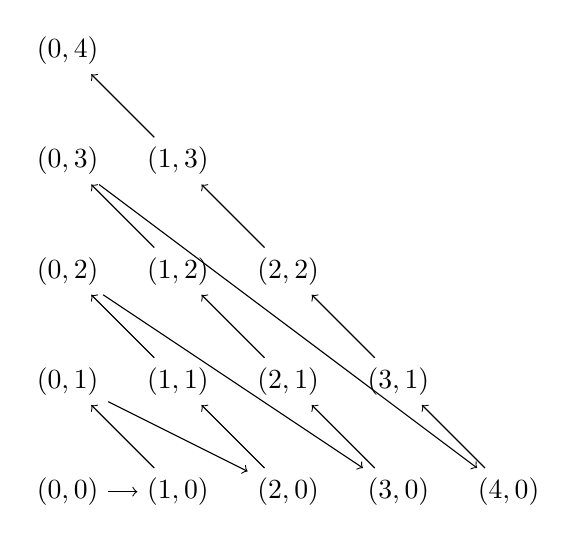
\begin{tikzpicture}[scale=1.4]
\node (0) at (0,0) {$(0,0)$};
\node (2) at (0,1) {$(0,1)$};
\node (5) at (0,2) {$(0,2)$};
\node (9) at (0,3) {$(0,3)$};
\node (14) at (0,4) {$(0,4)$};
\node (1) at (1,0) {$(1,0)$};
\node (4) at (1,1) {$(1,1)$};
\node (8) at (1,2) {$(1,2)$};
\node (13) at (1,3) {$(1,3)$};
\node (3) at (2,0) {$(2,0)$};
\node (7) at (2,1) {$(2,1)$};
\node (12) at (2,2) {$(2,2)$};
\node (6) at (3,0) {$(3,0)$};
\node (11) at (3,1) {$(3,1)$};
\node (10) at (4,0) {$(4,0)$};
\draw[->] (0) -- (1);
\draw[->] (1) -- (2);
\draw[->] (2) -- (3);
\draw[->] (3) -- (4);
\draw[->] (4) -- (5);
\draw[->] (5) -- (6);
\draw[->] (6) -- (7);
\draw[->] (7) -- (8);
\draw[->] (8) -- (9);
\draw[->] (9) -- (10);
\draw[->] (10) -- (11);
\draw[->] (11) -- (12);
\draw[->] (12) -- (13);
\draw[->] (13) -- (14);
\end{tikzpicture}
%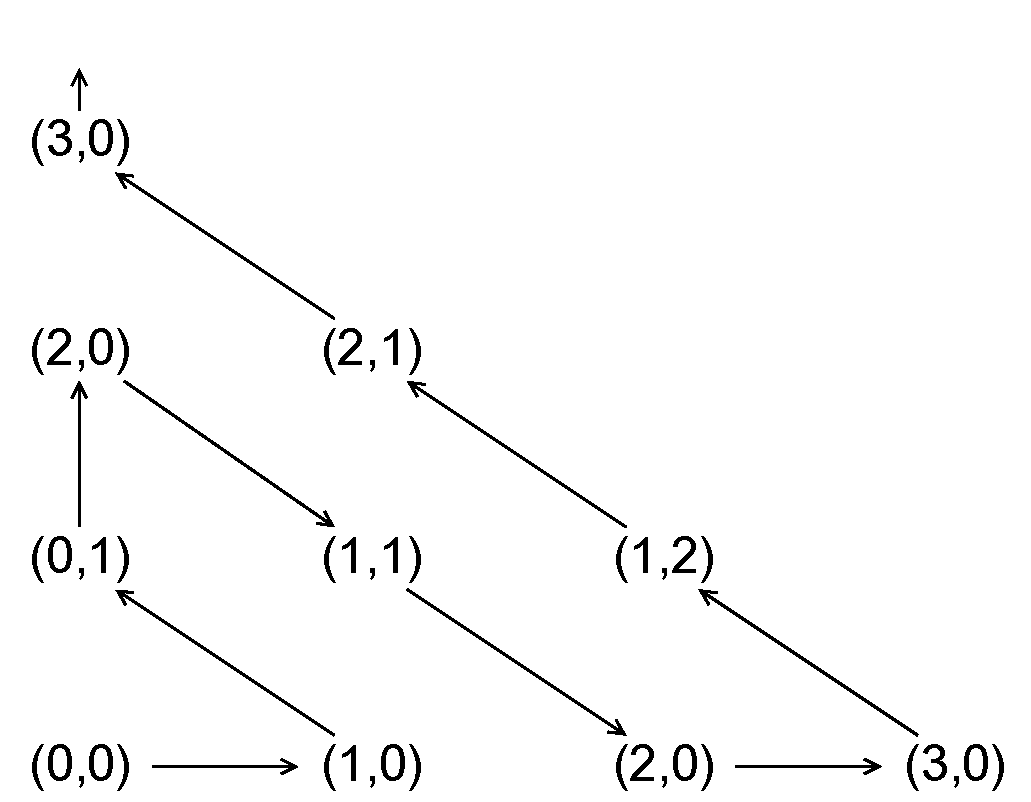
\includegraphics[width=0.5\linewidth]{images/figures/cantor1}
%\caption*{Die Pfeile deuten die Reihenfolge an, in der die Elemente von $\N\times\N$ abgezählt werden.}
\end{center}
\ %end{figure}
\end{proof}
\begin{lemma}{Vereinigung}
Jede Vereinigung von abzählbar vielen abzählbaren Mengen ist abzählbar. Konkret, jede Vereinigung von der Form
\[
\bigcup_{i\in\N}A_i
\]
ist abzählbar, wenn alle $A_i$'s abzählbar sind.
\end{lemma}
\begin{proof}{Abzählbarkeit Vereinigung}
Wir nehmen an, dass die Menge $\{A_i\mid i\in \N \}$ aus lauter abzählbaren Mengen besteht. Um zu zeigen, dass $\bigcup_{i\in N}A_i$ abzählbar ist, genügt es, aufgrund von Satz~\ref{satz:abzaehlbarTransitiv} und Satz~\ref{cantor1}, zu zeigen, dass es eine surjektive Funktion
\[
H:\N\times\N\to\bigcup_{i\in N}A_i
\]
gibt. Da für jede natürliche Zahl $i$ die Menge $A_i$ abzählbar ist, gibt es für jede natürliche Zahl $i$ auch eine surjektive Funktion $F_i:\N\to A_i$. Wir können die Vereinigungsmenge der $A_i$'s also wie folgt schreiben:
\begin{align*}
\bigcup_{i\in \N}A_i&=\{F_i(j)\mid i,j\in\N \}\\
&=\{F_i(j)\mid (i,j)\in\N\times\N \}.
\end{align*}
Daraus folgt, dass die Funktion
\[
H:\N\times\N\to \bigcup_{i\in N}A_i\phantom{abstand}\text{mit}\phantom{abstand} H(i,j)=F_i(j),
\]
die gesuchte surjektive Funktion ist.
\end{proof}

\begin{corollary}{Kartesisches Produkt}
Die Menge $\Z\times \Z$ ist abzählbar.
\end{corollary}
\begin{proof}{Abzählbarkeit Kartesisches Produkt}
Wir wissen bereits, dass die Menge $\N\times\N$ abzählbar ist. Daraus folgt, dass auch die Mengen
\begin{align*}
X&=\N\times\{-n\mid n\in \N\}\\
Y&=\{-n\mid n\in \N\}\times\N \\
Z&=\{-n\mid n\in \N\}\times\{-n\mid n\in \N\}
\end{align*}
abzählbar sind. Aus Satz~\ref{satz:countableUnion} folgt also, dass die Menge
\[
\Z\times\Z=(\N\times\N)\cup X\cup Y\cup Z
\]
abzählbar ist.
\end{proof}

\begin{corollary}{Rationale Zahlen}
Die Menge $\Q=\big\{\frac{x}{y}\mid x,y\in \Z\big\}$ der rationalen Zahlen (Brüche) ist abzählbar.
\end{corollary}
\begin{proof}{Abzählbarkeit Rationale Zahlen}
Da die Funktion
\[
F:\Z\times(\Z\setminus{\{0\}})\to \Q\phantom{abstand}\text{mit}\phantom{abstand}F(x,y)=\frac{x}{y}
\]
surjektiv ist, folgt die Behauptung aus Satz~\ref{satz:abzaehlbarTransitiv}.
\end{proof}



\begin{theorem}{Zweites Diagonalargument Cantor}
Die Menge aller unendlichen Binärsequenzen (Sequenzen aus Nullen und Einsen) ist überabzählbar.
\end{theorem}
\begin{proof}{Beweis zweites Diagonalargument}
Beweis durch Widerspruch. Wäre die Menge aller unendlichen Binärsequenzen abzählbar, dann gäbe es eine Liste von der Form\footnote{Natürlich ist die angedeutete Liste Beispielhaft und dient nur der Veranschaulichung unserer Konstruktion der Sequenz $b$. Die Sequenz $s_0$, beispielsweise, könnte auch mit dem Präfix $00000100$ oder irgend einer anderen Folge von Nullen und Einsen beginnen. }
\begin{center}
\begin{tabular}{c|l}
$\N$ & Binärsequenzen\\
\hline
$0$ & $s_0=01101011\cdots$\\
$1$ & $s_1=10010110\cdots$\\
$2$ & $s_2=00101001\cdots$\\
$\vdots$ & $\vdots$
\end{tabular}
\end{center}
in der alle unendlichen Binärsequenzen vorkommen. Wir konstruieren nun, ausgehend von dieser Liste, eine Binärsequenz $b$, die nicht in der Liste enthalten sein kann. Wir definieren $b$ wie folgt:
\begin{align*}
0\text{-tes Glied}&=b(0)=1-s_0(0)\\
1\text{-tes Glied}&=b(1)=1-s_1(1)\\
2\text{-tes Glied}&=b(2)=1-s_2(2)\\
&\vdots\\
n\text{-tes Glied}&=b(n)=1-s_n(n)\\
&\vdots
\end{align*}
Die Folge $b=110\cdots$ kann nicht in der Liste vorkommen, weil sie sich von jedem Element in der Liste in mindestens einem Glied unterscheidet (von der $n$-ten Sequenz unterscheidet sich $b$ im $n$-ten Glied). Dies steht im Widerspruch zu unserer Annahme, dass in der Liste alle unendlichen Binärsequenzen vorkommen.
\end{proof}


\begin{corollary}{Intervall}
Das Intervall $(0,1)=\{r\in\R\mid 0<r<1 \}$ ist überabzählbar. Insbesondere ist die Menge $\R$ der reellen Zahlen überabzählbar.
\end{corollary}
\begin{proof}{Überabzählbarkeit Intervall}
Die reellen Zahlen (in Binärdarstellung) im Intervall $(0,1)$, sind von der Form $0,\dots$ wobei $\dots$ für eine unendliche Binärsequenz steht. Daher steht das Intervall $(0,1)$ mit der Menge aller unendlichen Binärsequenzen in eins-zu-eins Korrespondenz. Die Behauptung folgt daher aus Theorem~\ref{thrm:cantor2}.
\end{proof}

\begin{corollary}{Potenzmenge}
Die Potenzmenge von $\N$ ist überabzählbar.
\end{corollary}
\begin{proof}{Überabzählbarkeit Potenzmenge}
Jede Teilmenge $A$ von $\N$ kann wie folgt durch eine Binärsequenz $\chi_A$ beschrieben werden:
\begin{align*}
\chi_A(n)=\begin{cases}
1&\text{falls } n\in A\\
0&\text{falls} n\notin A.
\end{cases}
\end{align*}
Daher folgt die Behauptung aus Theorem~\ref{thrm:cantor2}.
\end{proof}

\begin{corollary}{Menge aller Funktionen}
Die Menge aller Funktionen $F:\N\to\N$ ist überabzählbar.
\end{corollary}
\begin{proof}{Überabzählbarkeit der Menge aller Funktionen}
Die Menge der Binärsequenzen entspricht der Menge der Funktionen $F:\N\to\{0,1\}$. Daher folgt die Behauptung aus Theorem~\ref{thrm:cantor2}.
\end{proof}

\begin{corollary}{Unberechenbare Funktionen}
Es gibt Funktionen $F:\N\to\N$, die von keinem Java, C, C++, Fortran\dots Programm berechenbar sind. Solche Funktionen heissen \textit{unberechenbar}.
\end{corollary}




        \raggedcolumns
        \columnbreak
        s
        \raggedcolumns
        \columnbreak
        \subsection{Relationen, Funktionen und Graphen}


\begin{definition}{Tupel}
Es sei $n>0$ eine natürliche Zahl. Ein $n$\textit{-Tupel} ist ein Term von der Form
\[
(x_1,\dots,x_n).
\]
Für beliebige Tupel gilt:
\[
(x_1,\dots,x_n)=(y_1,\dots y_k):\Leftrightarrow n=k\land x_1=y_1\land\dots\land y_n=x_n.
\]
$2$-Tupel nennen wir \textit{Paare} und $3$-Tupel \textit{Tripel}.\\
\textit{Tupel} haben im Gegensatz zu Mengen mehr innere Struktur - die Reihenfolge und Wiederholung von Elementen sind wesentlich, sie sind gewissermassen die mathematische Entsprechung zu Listen und Arrays in der Informatik.
\end{definition}



\begin{definition}{Kartesisches Produkt}
Die Gesamtheit aller Tupel mit Elementen aus einer oder mehreren gegebenen Mengen nennt man kartesisches Produkt.\\
Es seien $A_1,\dots, A_n$ Mengen und $n\in\N$ mit $n>0$.
Das \textit{kartesische Produkt} von $A_1,\dots, A_n$, ist die Menge aller $n$-Tupel mit Einträgen aus den Mengen $A_1,\dots ,A_n$:
\begin{align*}
\prod_{i=1}^{n}A_i=\big\{(a_1,\dots,a_n)\mid a_1\in A_1\land\dots\land a_n\in A_n \big\}.
\end{align*}
\end{definition}

\begin{remark}
    Wir schreiben auch $A_1\times A_2\times \dots\times A_n$ für $\prod_{i=1}^nA_i$.\\ Insbesondere schreiben wir $X\times Y$ für das kartesische Produkt von zwei Mengen $X$ und $Y$, konkret heisst das:
    \[
    X\times Y:=\{(x,y)\mid x\in X\land y\in Y \}.
    \]
    Für das $n$-fache kartesisches Produkt $A\times A\times\dots\times A$ einer Menge $A$ mit sich selbst schreiben wir auch $A^n$.
    \end{remark}

    \begin{example}
        Die Menge der rationalen Zahlen
        \[
        \Q:=\left\{\frac{x}{y}\mid x\in \Z\land y\in\N\setminus\{0\}\right\}
        \]
        kann man als das kartesische Produkt
        \[
        \Z\times(\N\setminus\{0\})
        \]
        auffassen.
    \end{example}

\begin{definition}{Relation}
Eine $n$-stellige \textit{Relation} $R$ auf den Mengen $A_1,\dots A_n$ ist eine Menge von $n$-Tupeln aus $A_1\times\dots \times A_n$. Mit anderen Worten, die Relationen auf $A_1,\dots,A_n$ sind genau die Teilmengen
\begin{align*}
R\subseteq A_1\times\dots \times A_n.
\end{align*}
Ist $R$ eine $n$-stellige Relation und gilt $(x_1,\dots,x_n)\in R$, dann sagen wir, dass die Elemente $x_1,\dots,x_n$ zueinander in Relation $R$ stehen.
\tcblower
Eine $2$-stellige Relation $R\subseteq X\times Y$ heisst auch eine \textit{binäre Relation} auf den Mengen $X$ und $Y$. Ist $R$ eine binäre Relation, so schreiben wir auch $xRy$ für $(x,y)\in R$.
\end{definition}
\begin{comment}
\begin{example}\label{Bsp:Geraden}
    Wir betrachten die Relation $R_1$ von Beispiel~\ref{ex:Beispiel1relationen} auf $\{g,h,p,q,r\}$. Die Geraden $g,h,p,q,r$ sind wie im folgenden Bild gegeben:
    \begin{center}
    %\begin{framed}
    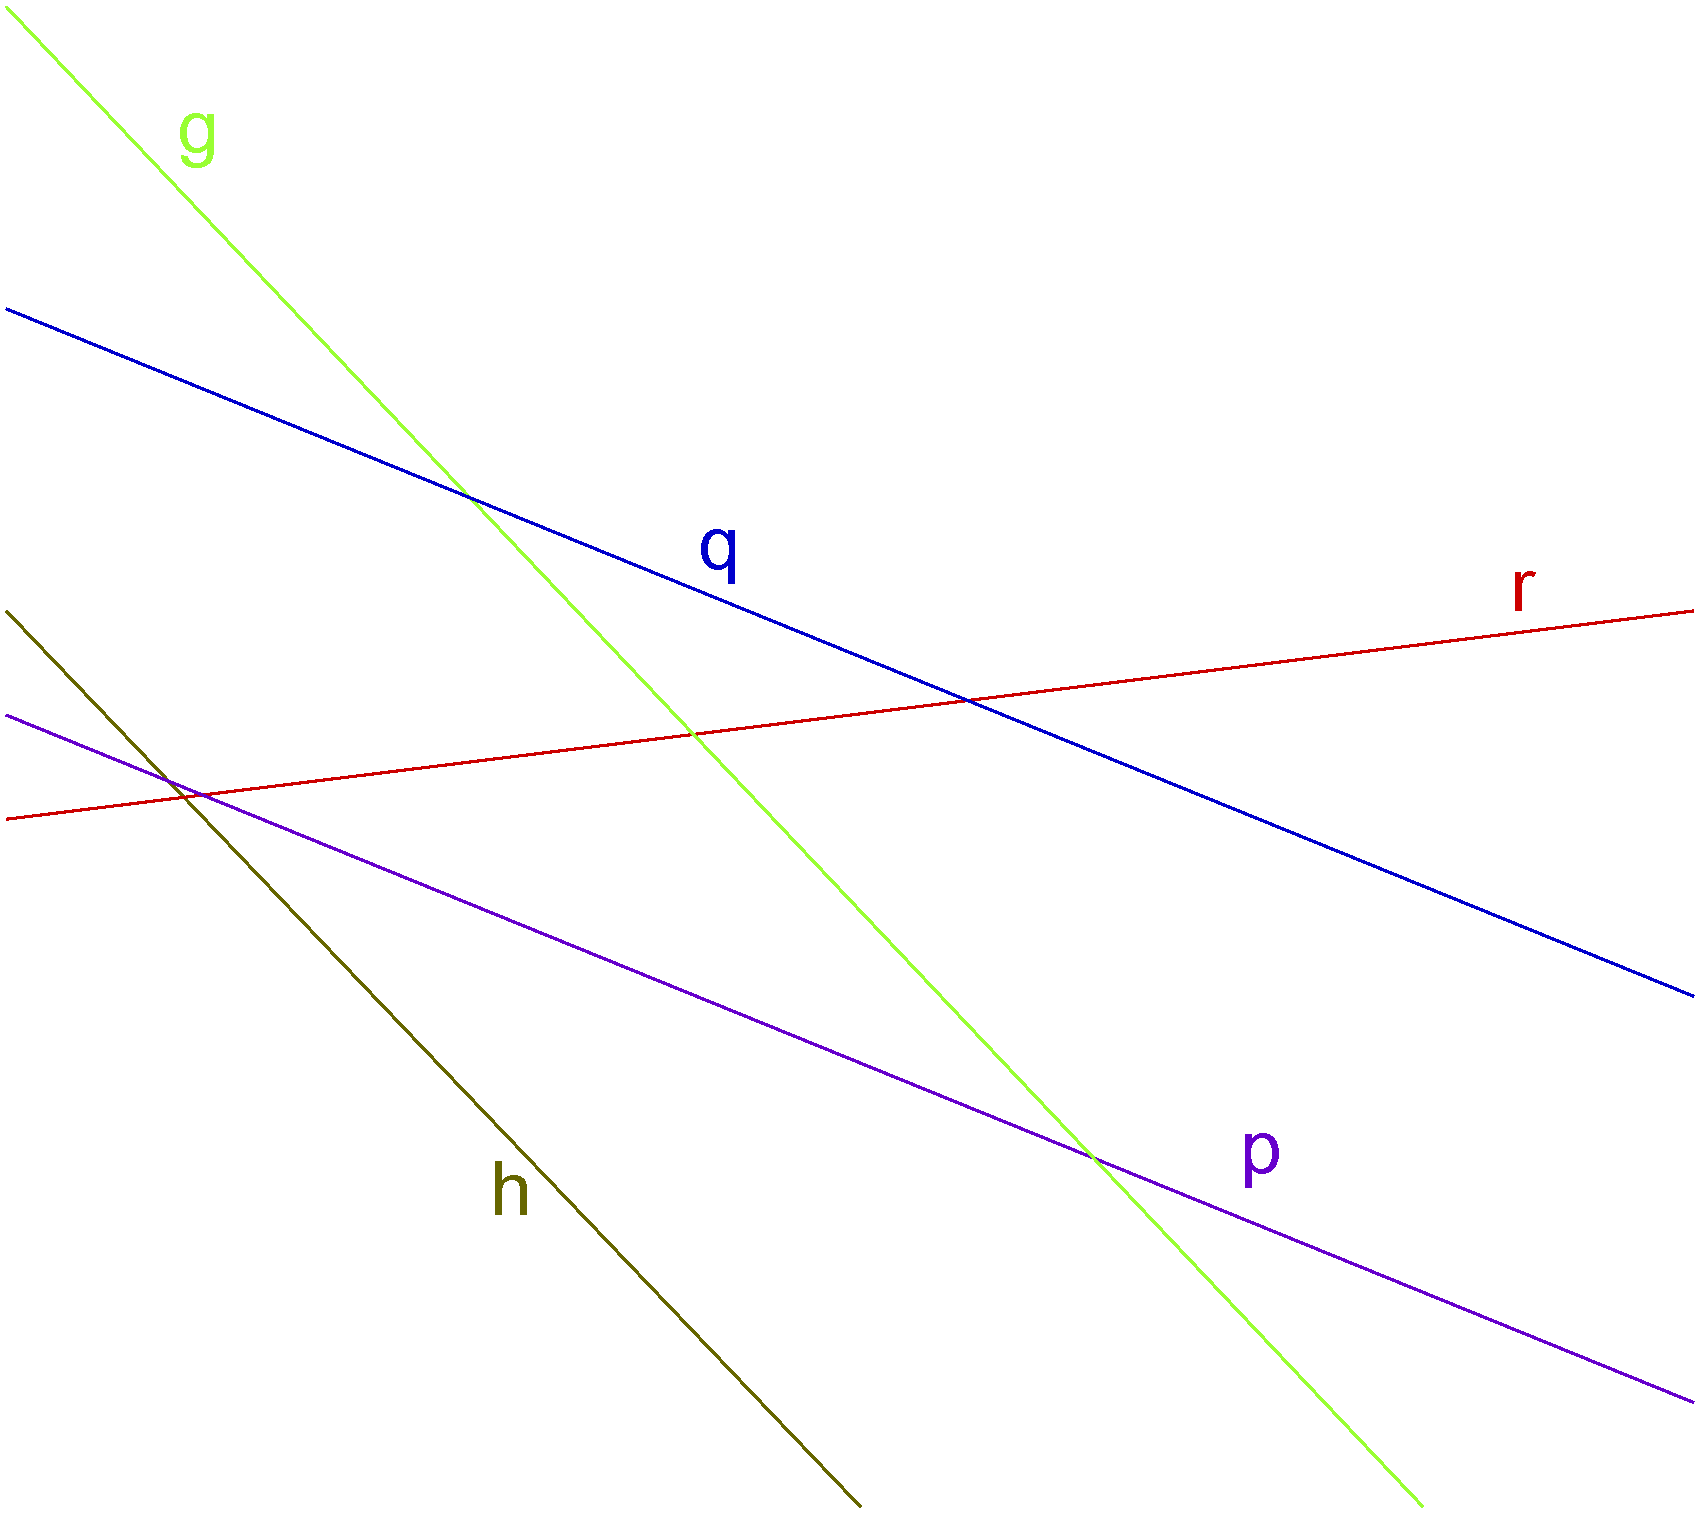
\includegraphics[width=0.5\linewidth]{images/figures/geraden}
    %\end{framed}
    \end{center}
    Offenbar gelten folgende Beziehungen:
    \begin{itemize}
    \item Die Gerade $g$ steht in Relation $R_1$ zu folgenden Geraden: $g$, $h$.
    \item Die Gerade $h$ steht in Relation $R_1$ zu folgenden Geraden: $g$, $h$.
    \item Die Gerade $p$ steht in Relation $R_1$ zu folgenden Geraden: $p$, $q$.
    \item Die Gerade $q$ steht in Relation $R_1$ zu folgenden Geraden: $p$, $q$.
    \item Die Gerade $r$ steht mit keiner anderen Geraden in Relation $R_1$.
    \end{itemize}
    Als Menge geschrieben, nimmt die Relation $R_1$ also folgende Gestalt an:
    \[
    R_1=\big\{(g,g),(g,h),(h,h),(h,g),(p,p),(p,q),(q,q),(q,p),(r,r)\big\}.
    \]
    Bildlich lässt sich die Relation als Tabelle darstellen:
    \begin{center}
    \begin{tabular}{ c | c c c c c }
    $r$&\xmark&\xmark&\xmark&\xmark&\cmark\\
    $q$&\xmark&\xmark&\cmark&\cmark&\xmark\\
    $p$&\xmark&\xmark&\cmark&\cmark&\xmark\\
    $h$&\cmark&\cmark&\xmark&\xmark&\xmark\\
    $g$&\cmark&\cmark&\xmark&\xmark&\xmark\\
    \hline
    &$g$&$h$&$p$&$q$&$r$
    \end{tabular}
    \end{center}
    Aus der Tabelle erhält man, ähnlich (gleich) wie im Fall von Funktionen und
    Funktionsgraphen, den Relationsgraph von $R_1$:
    \begin{center}
    \begin{tabular}{ c | c c c c c }
    $r$&&&&&\cellcolor{black}\\
    $q$&&&\cellcolor{black}&\cellcolor{black}&\\
    $p$&&&\cellcolor{black}&\cellcolor{black}&\\
    $h$&\cellcolor{black}&\cellcolor{black}&&&\\
    $g$&\cellcolor{black}&\cellcolor{black}&&&\\
    \hline
    &$g$&$h$&$p$&$q$&$r$
    \end{tabular}
    \end{center}
\end{example}
\end{comment}



\begin{definition}{Gerichteter Graph}
    Ein \textit{(gerichteter) Graph} ist ein Paar $G=(V,E)$ bestehend aus einer Menge $V$ (Knotenmenge)
    und einer binären Relation $E\subseteq V\times V$ (Kantenmenge).
\end{definition}






\subsection{Ordnungs- und Äquivalenzrelationen}

\begin{definition}{Eigenschaften von Relationen}
    Eine binäre Relation $R$ auf einer Menge $X$ heisst:
    \begin{itemize}
    \item \textit{Reflexiv}, wenn für alle $x\in X$
    \[
    xRx
    \]
    
    \item \textit{Symmetrisch}, wenn für alle $x,y\in X$
    \[
    xRy\,\Rightarrow\, yRx
    \]
    
    \item \textit{Antisymmetrisch}, wenn für alle $x,y\in X$
    \[
    xRy\land yRx\,\Rightarrow x=y
    \]
    
    \item \textit{Transitiv}, wenn für alle $x,y,z\in X$
    \[
    xRy\land yRz\,\Rightarrow \, xRz
    \]
    
    \end{itemize}
    \end{definition}




    \subsection*{Äquivalenzrelationen}

    Äquivalenzrelationen sind in einem gewissen Sinn verallgemeinerte Gleichheitsrelationen. Sie werden dazu verwendet, (im Sinn der Relation) ähnliche Objekte miteinander zu identifizieren und als ``gleich'' zu behandeln.

    \begin{definition}{Äquivalenzrelation}
    \textit{Äquivalenzrelationen} sind reflexive, symmetrische und transitive Relationen.
    \end{definition}


    \begin{definition}{Äquivalenzklasse}
    Es sei $R$ eine Äquivalenzrelation auf einer Menge $X$ und $x\in X$. Die \textit{Äquivalenzklasse} $[x]_R$ von $x$ bezüglich $R$ ist die Menge aller Elemente von $X$, die zu $x$ in Relation $R$ stehen:
    \[
    [x]_R:=\{y\in X\mid xRy \}
    \]
    Jedes Element einer Äquivalenzklasse nennen wir einen \textit{Repräsentanten} der entsprechenden Äquivalenzklasse. Die \textit{Faktormenge} $\faktor{X}{R}$ \textit{von} $X$ \textit{modulo} $R$ ist die Menge aller Äquivalenzklassen:
    \[
    \faktor{X}{R}:=\big\{ [x]_R\mid x\in X \big\}
    \]
    \end{definition}

    
    \begin{lemma}{Äquivalente Elemente}
    Ist $\sim $ eine Äquivalenzrelation auf einer Menge $X$ und gilt $x,y\in X$ mit $x\sim y$, dann gilt $[x]_\sim=[y]_\sim$. Mit anderen Worten, äquivalente Elemente repräsentieren stets dieselbe Äquivalenzklasse.
    \end{lemma}
    
    \begin{proof}{Äquivalenz zeigen}
    Seien $X,\sim,x,y$ wie in der Behauptung. Um zu zeigen, dass $[x]_\sim=[y]_\sim$ gilt, genügt es nachzuweisen, dass $x\sim z\Leftrightarrow y\sim z$ für beliebige $z\in X$ gilt. Wir nehmen $x\sim y$ an, dann gilt
    \begin{align*}
    y\sim z\Rightarrow x\sim y\land y\sim z \stackrel{\text{Transitivität}}{\Longrightarrow} x\sim z
    \end{align*}
    und
    \[
    x\sim z\Rightarrow x\sim y\land x\sim z\stackrel{\text{Symmetrie}}{\Longrightarrow} y\sim x\land x\sim z\stackrel{\text{Transitivität}}{\Longrightarrow} y\sim z,
    \]
    wie gewünscht.
    \end{proof}
    
    \begin{corollary}{Elemente als Repräsentanten}
    Ist $\sim $ eine Äquivalenzrelation auf $X$ und sind $x,y\in X$ mit $x\in[y]_\sim$, dann gilt $[x]_\sim=[y]_\sim$. Mit anderen Worten, jedes Element einer Äquivalenzklasse ist auch ein Repräsentant dieser Äquivalenzklasse.
    \end{corollary}
    
    \begin{proof}{Äquivalenz zeigen Variante 2}
    Es seien $X,\sim,x$ und $y$ wie in der Behauptung. Aus $x\in[y]_\sim$ folgt $y\sim x$. Die Behauptung folgt nun aus Lemma~\ref{lm:sim gleiche klasse}.
    \end{proof}

    \begin{lemma}{Disjunktheit Equivalenzklassen}
    Ist $\sim $ eine Äquivalenzrelation auf $X$ und sind $x,y\in X$ mit $[x]_\sim\neq[y]_\sim$, dann gilt $[x]_\sim\cap[y]_\sim=\varnothing$.
    Mit anderen Worten, verschiedene Äquivalenzklassen sind immer disjunkt.
    \end{lemma}
    
    \begin{proof}{Disjunktheit von Äquivalenzklassen zeigen}
    Es seien $X,\sim,x$ und $y$ wie in der Behauptung. Wir zeigen die Kontraposition, d.h.
    \[
    [x]_\sim\cap[y]_\sim\neq\varnothing\Rightarrow [x]_\sim=[y]_\sim.
    \]
    Es gelte also $[x]_\sim\cap[y]_\sim\neq\varnothing$, es gibt daher ein $z\in [x]_\sim\cap[y]_\sim$. Daraus folgt, dass $x\sim z\land y\sim z$ gilt und wegen der Transitivität und der Symmetrie von $\sim$ folgt sofort $x\sim y$. Die Behauptung folgt nun aus Lemma~\ref{lm:sim gleiche klasse}.
    \end{proof}


    \begin{lemma}{Equivalenzklassen Partition}
    Ist $\sim$ eine Äquivalenzrelation auf einer Menge $X$, dann ist die Faktormenge $\faktor{X}{\sim}$ eine Partition von $X$.
    \end{lemma}
    
    \begin{proof}{Eigenschaften von Äquivalenzrelationen beweisen}
    Es sei $\sim$ eine beliebige Äquivalenzrelation auf einer Menge $X$. Wir müssen folgende Punkte verifizieren:
    \begin{enumerate}
    \item\label{a} Die Äquivalenzklassen sind alle nichtleer.
    \item\label{2} Die Äquivalenzklassen sind paarweise disjunkt.
    \item\label{3} Es gilt
    \[
    \bigcup_{x\in X}[x]_{\sim}=X.
    \]
    \end{enumerate}
    Der erste Punkt folgt aus der Definition von der Faktormenge (die Äquivalenzklassen sind via ihrer Repräsentanten definiert). Die Tatsache, dass die Äquivalenzklassen paarweise disjunkt sind, ist genau die Aussage von dem Satz Disjunktheit von Äquivalenzklassen. Wir brauchen also bloss noch den letzten Punkt zu verifizieren. Dies folgt, da für jedes $z\in X$, wegen der Reflexivität, $z\sim z$ und somit
    \[
    z\in[z]_\sim\subseteq\bigcup_{x\in X}[x]_\sim
    \]
    gilt.
    \end{proof}



    \begin{lemma}{Partition induziert Äquivalenzrelation}
    Ist $P=\{A_i\mid i\in I\}$ eine Partition von der Menge $X$, dann ist die Relation $\sim$, gegeben durch
    \[
    x\sim y:\Leftrightarrow \exists i\in I\,(x\in A_i\land y\in A_i),
    \]
    eine Äquivalenzrelation auf $X$. Zusätzlich gilt
    \[
    \faktor{X}{\sim}=P.
    \]
    \end{lemma}
    
    \begin{proof}{Äquivalenzrelation verifizieren}
    Zuerst zeigen wir, dass die Relation $\sim$ unter den gegebenen Umständen eine Äquivalenzrelation ist.
    \begin{itemize}
    \item \textbf{Reflexivität}: Sei $x\in X$  beliebig. Wir müssen zeigen, dass $x\sim x$ gilt. Da $P=\{A_i\mid i\in I\}$ eine Partition von $X$ ist, gibt es ein $i\in I$ mit $x\in A_i$, daraus folgt sofort $x\sim x$.
    \item \textbf{Symmetrie}: Es gelte $x\sim y$. Wir müssen $y\sim x$ zeigen. Aus $x\sim y$ folgt, dass es ein $i\in I$ mit $x\in A_i\land y\in A_i$ gibt, dies ist offensichtlich äquivalent zu $y\sim x$.
    \item \textbf{Transitivität}: Es gelte $x\sim y\land y\sim z$. Wir müssen $x\sim z$ zeigen. Aus $x\sim y\land y\sim z$ folgt, dass es $i,j\in I$ gibt so, dass $x,y\in A_i$ und $y,z\in A_j$ gilt. Da $P=\{A_i\mid i\in I\}$ eine Partition ist, kann $y $ nicht in zwei verschiedenen Blöcken enthalten sein, es gilt daher $i=j$ und somit $x\sim z$.
    \end{itemize}
    Dass die Äquivalenzklassen von $\sim$ genau den Blöcken von $P$ entsprechen ist sofort klar, wenn man beachtet, dass zwei Elemente genau dann äquivalent sind, wenn sie im selben Block von $P$ liegen.
    \end{proof}

    \begin{lemma}{Äquivalenzrelationen: Verallgemeinerte Gleichheit}
    Für jede Relation $\sim$ auf einer Menge $X$ sind folgende beiden Aussagen äquivalent.
    \begin{enumerate}
    \item[1.] Die Relation $\sim$ ist eine Äquivalenzrelation.
    \item[2.] Es gibt eine Menge $Y$ und ein Funktion $F:X\to Y$ so, dass für alle $x,y\in X$
    \[
    x\sim y\Leftrightarrow F(x)=F(y)
    \]
    gilt.
    \end{enumerate}
    \end{lemma}
    
    \begin{proof}{Gleichheit in Äquivalenzrelationen zeigen}
    Wenn $\sim$ eine Äquivalenzrelation auf der Menge $X$ ist, dann erfüllt die Abbildung
    \[
    F:X\to\mathcal{P}(X)\phantom{abstand}\text{mit} \phantom{abstand} F(x)=[x]_\sim
    \]
    alle geforderten Eigenschaften. Ist umgekehrt eine Funktion $F:X\to Y$ wie in der Behauptung gegeben, dann gilt für die Relation $\sim$ Folgendes:
    \begin{itemize}
    \item\textbf{Reflexivität} gilt, da für jedes Element $x\in X$ trivialerweise $F(x)=F(x)$ gilt.
    \item \textbf{Symmetrie} folgt, da für beliebige Elemente $x,y\in X$
    \[
    x\sim y\Rightarrow F(x)=F(y)\Rightarrow F(y)=F(x)\Rightarrow y\sim x
    \]
    gilt.
    \item\textbf{Transitivität} folgt, da für beliebige Elemente $x,y,z\in X$
    \[
    x\sim y\land y\sim z\Rightarrow F(x)=F(y)\land F(y)=F(z)\Rightarrow F(x)=F(z)\Rightarrow  x\sim z
    \]
    gilt.
    \end{itemize}
    \end{proof}


    \subsection*{Ordnungsrelationen}

    \begin{definition}{Minimale Elemente}
    Es sei $R$ eine binäre Relation auf der Menge $M$.
    \begin{itemize}
    \item Zwei Elemente $x,y\in M$ heissen $R$-\textit{unvergleichbar}, falls weder $xRy$ noch $yRx$ gilt.
    \item Ein Element $x\in X$ einer Teilmenge $X\subseteq M$ von $M$ heisst $R$-\textit{minimal in $X$}, falls es kein anderes Element $y\in X$ mit $yRx$ gibt.
    \item  Ein Element $x\in X$ einer Teilmenge $X\subseteq M$ von $M$ heisst $R$-\textit{maximal in $X$}, falls es kein anderes Element $y\in X$ mit $xRy$ gibt.
    \end{itemize}
    Wenn keine Missverständnisse zu befürchten sind, dann schreiben wir anstelle von $R$-minimal, $R$-maximal und $R$-unvergleichbar auch einfach minimal, maximal und unvergleichbar.
    \end{definition}


    \begin{definition}{Ordnungsrelation}
    Es sei $R$ eine binäre Relation auf der Menge $M$.
    \begin{itemize}
    \item $R$ ist eine \textit{Präordnung} auf $M$, wenn $R$ reflexiv und transitiv ist.
    \item $R$ ist eine \textit{Halbordnung} auf $M$, wenn $R$ reflexiv, antisymmetrisch und transitiv ist.
    \item $R$ ist eine \textit{totale oder lineare Ordnung} auf $M$, wenn $R$ eine Halbordnung ist und keine $R$-unvergleichbaren Elemente existieren.
    \item $R$ ist eine \textit{Wohlordnung} auf $M$, wenn $R$ eine totale Ordnung auf $M$ ist so, dass jede Teilmenge $X\neq\varnothing$ von $M$ (mindestens) ein $R$-minimales Element enthält.
    \end{itemize}
    \end{definition}


    \begin{example}~
    \begin{itemize}
    \item Die Relation $\leq$ auf der Menge $\R$ ist eine totale Ordnung, die aber keine Wohlordnung ist (die Menge $\{x\in\R\mid 0<x<1\}$ hat kein kleinstes Element). Auf der Menge $\N$ ist $\leq$ eine Wohlordnung\footnote{Ein Beweis dazu kommt im nächsten Kapitel.}. Auf der Menge $\Z$ ist die Relation $\leq$ keine Wohlordnung. Wieso?
    \item Ist $A$ eine Menge von Mengen, dann ist die Teilmengenrelation $\subseteq$ eine Halbordnung.
    \item Die Teilerrelation $T$ auf der Menge $\Z$ ist eine Halbordnung aber keine totale Ordnung. Die Elemente $7$ und $5$ sind $T$-unvergleichlich.
    \end{itemize}
    \end{example}

    \begin{definition}{Transitiver Abschluss}
        Es sei $R$ eine (bin\"are) Relation.
        \begin{itemize}
            \item Als \textit{transitiven Abschluss} von $R$ bezeichnet man die kleinste
            (bezüglich $\subseteq$) transitive Relation, die $R$ als Teilmenge enthält,
            sie wird mit $R^+$ notiert.
            \item Die kleinste Relation, die $R^+$ enthält und reflexiv ist, nennt man den
            \textit{reflexiv-transitiven Abschluss} von $R$, sie wird mit $R^*$ bezeichnet.
        \end{itemize}
    \end{definition}

    \begin{remark}
        F\"ur eine beliebige (bin\"are) Relation $R$ gilt genau dann $xR^*y$, wenn es
        eine endliche Folge $x=k_1,\dots,k_n=y$ gibt, so dass $k_iRk_{i+1}$ f\"ur alle
        Indices $i=1,\dots,n-1$ gilt. Es gilt also genau dann $xR^*y$, wenn es eine Folge von
        Elementen gibt, die mit $x$ beginnt, mit $y$ endet und deren Elemente alle der Reihe
        nach in Relation $R$ zueinander stehen. Ist $G=(V,E)$ ein Graph, dann bedeutet
        $xE^*y$, dass in $G$ ein Pfad von $x$ nach $y$ existiert.
    \end{remark}

    \begin{definition} {Pfad und Zyklus}
        Ein \textit{Weg} oder \textit{Pfad} in einem Graph $G=(V,E)$ ist eine endliche Folge
        $k_1,\dots,k_n\in V$ von Knoten, so dass $k_iEk_{i+1}$ f\"ur alle Indices
        $i=1,\dots,n-1$ gilt. Die Knoten $k_1$ und $k_n$ bezeichnet man als \textit{Anfangs-}
        und \textit{Endpunkt} des Pfades. Gilt zusätzlich $k_1=k_n$, dann spricht man von einem \textit{Zyklus}.
    \end{definition}


    \begin{definition}{Topologische Sortierung}
        Es sei $M$ eine endliche Menge und $G=(M,E)$ ein DAG. Eine lineare Ordnung $\preceq\subseteq M\times M$ ist eine \textit{topologische Sortierung} von $G$, wenn für alle $a,b\in M$
        \begin{align*}
        a E^* b  \Rightarrow a\preceq b
        \end{align*}
        gilt.
    \end{definition}

    \begin{lemma}{Topologische Sortierung DAG}
        Jeder endliche DAG besitzt (mindestens) eine topologische Sortierung.
    \end{lemma}
    
    \begin{proof}{Topologische Sortierung DAG}
        Wir bemerken zuerst, dass jeder endliche DAG $G=(V,E)$ minimale Elemente bezüglich der Relation $E$ besitzt (wieso?). Weiter bemerken wir, dass jeder DAG, von dem ein minimaler Knoten (zusammen mit den von diesem Knoten ausgehenden Pfeilen) entfernt wird, wieder ein DAG ist (entfernen von Knoten und Verbindungen kann keine neuen Zyklen erzeugen). Aus diesen Beobachtungen folgt, dass folgender Algorithmus eine topologische Sortierung für jeden endlichen DAG generiert:
        \begin{enumerate}
            \item Wenn $G=(V,E)$ nicht leer ist, dann wähle ein bezüglich $E$ minimales Element $x\in V$ (Wenn $V$ leer ist, terminiere).
            \item Wiederhole die erste Instruktion mit $G'=(V\setminus \{x\},\{(a,b)\in E\mid a\neq x \})$ (d.h. erstelle den DAG $G'$ durch Entfernen von $x$ aus $V$ und entfernen von allen von $x$ ausgehenden Kanten in $E$).
        \end{enumerate}
    Die Reihenfolge, mit der die Elemente entfernt werden, entspricht einer topologischen Sortierung.
    \end{proof}


    \begin{lemma}{Halbordnung DAG}
        Folgende Aussagen sind äquivalent:
        \begin{enumerate}
            \item $(V,E\setminus \Delta_V)$ ist ein DAG.
            \item $E^*$ ist eine Halbordnung auf $V$.
        \end{enumerate}
    \end{lemma}
    
    \begin{proof}{Halbordnung DAG}
        $a)\Rightarrow b)$: Es sei $(V,E)$ ein DAG. Weil $E^*$ nach Definition bereits
        reflexiv und transitiv ist, müssen wir bloss noch zeigen, dass $E^*$
        antisymmetrisch ist. Gilt $xE^*y$, $yE^*x$ und $x\neq y$, dann gibt es
        Pfade $x,a_1,\dots,a_n,y$ und $y,b_1,\dots,b_m,x$ in $(V,E\setminus \Delta_V)$ (eventuell ist das Entfernen von Wiederholungen nötig, vgl. Wandtafel) und daher auch
        einen Zyklus $x,a_1,\dots,a_n,y,b_1,\dots,b_m$. Die Behauptung folgt per
        Kontraposition.

        $b)\Rightarrow a)$: Wenn $E^*$ eine Halbordnung ist, dann existieren aufgrund der
        Antisymmetrie keine Zyklen mit mehr als einem Knoten in $(V,E)$, daher existieren in
        $(V,E\setminus\Delta_V)$ gar keine Zyklen (vgl. Bild Wandtafel).
    \end{proof}

    \begin{corollary}{Halbordnung - lineare Ordnung}
        Jede endliche Halbordnung kann zu einer linearen Ordnung erweitert werden. Formal, zu jeder Halbordnung $\preceq$ auf einer Menge $M$ gibt es eine lineare Ordnung $\ll$ auf $M$, so dass
        \begin{align*}
        a\preceq b \Rightarrow a\ll b
        \end{align*}
        gilt.
    \end{corollary}
    
    \begin{proof}{Halbordnung - lineare Ordnung}
        Wir haben bereits gesehen, dass der Graph $G=(M,\preceq\setminus\Delta_M)$ ein DAG ist. Jede topologische Sortierung von $G$ erfüllt die Behauptung.
    \end{proof}


    \begin{lemma}{Wohlordnung - kleinstes Element}
    Ist $\preceq$ eine Wohlordnung auf einer Menge $M$, dann gibt es keine unendlich absteigende Folge
    \[
    a_0\succeq a_1\succeq\dots\succeq a_n\succeq a_{n+1}\succeq\dots
    \]
    von verschiedenen Elementen aus $M$.
    \end{lemma}
    
    \begin{proof}{Wohlordnung - kleinstes Element}
    Gibt es eine absteigende Folge $a_0,a_1,\dots$ wie in der Behauptung, dann ist die Menge
    \[
    \{a_i\mid i\in M\}
    \]
    eine Teilmenge von $M$, die kein $\preceq$-minimales Element besitzt. Die Relation $\preceq$ kann also in diesem Fall keine Wohlordnung sein. Die Behauptung folgt durch Kontraposition.
    \end{proof}


    \begin{example}
        Geben Sie zwei $\leq^*$ unvergleichbare Funktionen $f$ und $g$ an.
        \tcblower
        Zum Beispiel
            \begin{align*}
                f(n) =  \begin{cases}
                            1&\text{ falls $n$ gerade}\\
                            0&\text{ sonst}
                        \end{cases}
            \end{align*}
            und
            \begin{align*}
                g(n) =  \begin{cases}
                            0&\text{ falls $n$ ungerade}\\
                            1&\text{ sonst}
                        \end{cases}
            \end{align*}
    \end{example}

    \begin{definition}{Hasse-Diagramm}
    Es sei $\preceq$ eine Halbordnung auf einer Menge $M$. Das \textit{Hasse-Diagramm} von $R$ ist eine vereinfachte Darstellung des Graphen $(M,\preceq)$.
    \begin{itemize}
    \item Die Richtung eines Pfeiles $a\to b$ für Elemente $a,b\in M$ wird dadurch zum Ausdruck gebracht, dass sich der Knoten $b$ oberhalb von $a$ befindet.
    \item Pfeile zwischen zwei Punkten $a,b$ werden gelöscht, wenn es einen weiteren Punkt $c$ mit $a\preceq c\preceq b$ gibt.
    \item Pfeile, die von einem Punkt auf denselben Punkt zeigen (Schleifen), werden weggelassen.
    \end{itemize}
    \end{definition}

  

    \section{Rekursive Strukturen und die natürlichen Zahlen}
        \input{contents/Chapters/4_Rekursive_Strukturen/4.1_Struktur_natürliche_Zahlen}
        %\section{Vom Induktionsbeweis zum rekursiven Algorithmus}

\begin{example}[Türme von Hanoi]~
\begin{center}
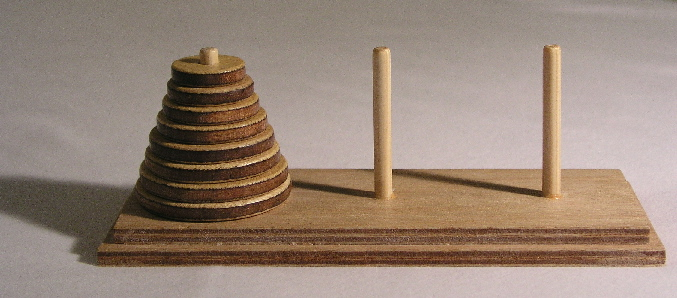
\includegraphics[width=0.8\linewidth]{images/figures/hanoi}
\end{center}
\begin{quote}
``Die Türme von Hanoi''\footnote{Beschreibung und Bild von Wikipedia.} ist ein Geduldspiel. Das Spiel besteht aus drei gleich grossen Stäben A, B und C, auf die mehrere gelochte Scheiben gelegt werden, alle verschieden gross. Zu Beginn liegen alle Scheiben auf Stab A, der Grösse nach geordnet, mit der grössten Scheibe unten und der kleinsten oben. Ziel des Spiels ist es, den kompletten Scheiben-Stapel von A nach C zu versetzen.
Bei jedem Zug darf die oberste Scheibe eines beliebigen Stabes auf einen der beiden anderen Stäbe gelegt werden, vorausgesetzt, dort liegt nicht schon eine kleinere Scheibe. Folglich sind zu jedem Zeitpunkt des Spieles die Scheiben auf jedem Feld der Grösse nach geordnet.
\end{quote}
Wir wollen beweisen, dass ``die Türme von Hanoi'' mit beliebig vielen Scheiben erfolgreich gespielt werden können.
\begin{proof} Wir benutzen ein Induktionsargument ($n$ sei die Anzahl Scheiben):
\begin{itemize}
\item \textbf{Verankerung $n=0$:} Dieser Fall ist trivial, da es keine Scheiben zu bewegen gibt.
\item \textbf{Induktionsschritt $n\to n+1$:} Wir betrachten das Spiel mit $n+1$ Scheiben. Nach Induktionsvoraussetzung gibt es eine Lösungsstrategie für das Spiel mit nur $n$ Scheiben. Diese Strategie können wir offensichtlich dazu verwenden, um alle bis auf die grösste Scheibe auf den Stab B zu verschieben. Nun können wir die grösste Scheibe auf den Stab $C$ verschieben, um anschliessend nochmal die Strategie für das Spiel mit $n$ Scheiben anzuwenden und alle kleineren Scheiben auf den Stab C zu bewegen. Das Spiel ist somit auch für $n+1$ Scheiben lösbar. \qedhere
\end{itemize}
\end{proof}
\begin{remark}
Der Beweis, dass die Türme von Hanoi für beliebige $n$ gelöst werden können, ist mehr als nur eine Argumentationskette, die dazu geeignet ist jemanden davon zu überzeugen, dass es tatsächlich \textit{irgendwie möglich sein muss} das Spiel zu gewinnen. Es steckt viel mehr in diesem Beweis; der Beweis gibt einen konkreten Algorithmus (rekursiv) vor, wie das Spiel erfolgreich gespielt werden kann. Wir betrachten eine Implementierung dieser Lösungsstrategie in Java.


\lstset{language=Java}
\begin{framed}
\begin{lstlisting}
// x-viele Scheiben von A nach B verschieben:
// Falls x=0, dann ist nichts zu tun.
// Sonst, zuerst die oberen (x-1) Scheiben von A nach C
// verschieben,
// dann die groesste Scheibe von A nach B verschieben
// und schliesslich alle anderen Scheiben von C nach B
// verschieben
public class HanoiSolver{

    public String solve(int size){
        return AC(size);
    }

    private String AB(int x){
        if (x==0) return "";
        return AC(x-1)+" AB "+CB(x-1);
    }

    private String AC(int x){
            if (x==0) return "";
            return AB(x-1)+" AC "+BC(x-1);
    }

    private String BC(int x){
            if (x==0) return "";
            return BA(x-1)+" BC "+AC(x-1);
    }

    private String BA(int x){
            if (x==0) return "";
            return BC(x-1)+" BA "+CA(x-1);
    }

    private String CB(int x){
            if (x==0) return "";
            return CA(x-1)+" CB "+AB(x-1);
    }

    private String CA(int x){
            if (x==0) return "";
            return CB(x-1)+" CA "+BA(x-1);
    }
}
\end{lstlisting}
\end{framed}
und die kurze Fassung:
\begin{framed}
\begin{lstlisting}
public class HanoiSolverCompact{

    public String solve(int size){
        return hanoi("A","C","B",size);
    }

    private String hanoi(String x,String y,String z,int n){
        if(n==0) return "";
        return hanoi(x,z,y,n-1)+" "+x+y+hanoi(z,y,x,n-1);
    }
}
\end{lstlisting}
\end{framed}

%\begin{lstlisting}
%let rec AB x =
%    if x=0 then []
%    else (CB (x-1))@(('A','B')::(AC (x-1)))
%
%and AC x =
%    if x=0 then []
%    else (BC (x-1))@(('A','C')::(AB (x-1)))
%
%and BC x =
%    if x=0 then []
%    else (AC (x-1))@(('B','C')::(BA (x-1)))
%
%and BA x =
%    if x=0 then []
%    else (CA (x-1))@(('B','A')::(BC (x-1)))
%
%and CB x =
%    if x=0 then []
%    else (AB (x-1))@(('C','B')::(CA (x-1)))
%
%and CA x =
%    if x=0 then []
%    else (BA (x-1))@(('C','A')::(CB (x-1)))
%
%\end{lstlisting}
\end{remark}
\end{example}


\begin{example}\label{bsp:plättli}
Ist es immer möglich ein ``gelochtes $n\times n$-Quadrat''
\begin{center}
\begin{tabular}{ | c | c | c | c | c  | c | c | c | }
\hline
&&&&&&&\\
\hline
&&&&&&&\\
\hline
&&&&&&&\\
\hline
&&&&&&&\\
\hline
&&&&&&\cellcolor{black}&\\
\hline
&&&&&&&\\
\hline
&&&&&&&\\
\hline
&&&&&&&\\
\hline
\end{tabular}
\end{center}

mit Flächen von der Form
\begin{tabular}{ c c }
&\cellcolor{black}\\
\cellcolor{black}&\cellcolor{black}
\end{tabular}
``passgenau'' zu überdecken? Ja, wenn $n$ eine Zweierpotenz ist. Wir können diese Behauptung durch Induktion wie folgt beweisen:  Wir nehmen an, dass das ``gelochte Quadrat'' eine Seitenlänge von $2^n$ hat.
\begin{itemize}
\item Verankerung ($n=0$): Wenn $n=0$, dann besteht das gelochte Quadrat nur aus einem Loch. Wir können das Quadrat (ohne etwas zu tun) überdecken.
\item Hat das Quadrat die Seitenlänge $2^{n+1}$, dann zerlegen wir es in vier gleich grosse Quadranten, die alle die Seitenlänge $2^n$ haben. Wir platzieren eine der Flächen wie unten angedeutet (rot).
\begin{center}
\begin{tabular}{ | c | c | c | c !{\color{red}\vrule} c  | c | c | c | }
\hline
&&&&&&&\\
\hline
&&&&&&&\\
\hline
&&&&&&&\\
\hline
&&&\cellcolor{red}&\cellcolor{red}&&&\\
\arrayrulecolor{red}\hline
\arrayrulecolor{black}&&&\cellcolor{red}&&&&\\
\hline
&&&&&&\cellcolor{black}&\\
\hline
&&&&&&&\\
\hline
&&&&&&&\\
\hline
\end{tabular}
\end{center}
Nun sind alle Quadranten ein ``gelochtes Quadrat'' der Seitenlänge $2^n$. Wir können also nach Induktionsvoraussetzung alle Quadranten passgenau belegen.
\end{itemize}
\end{example}

\begin{example}
Implementieren Sie (ausgehend vom Beispiel~\ref{bsp:plättli}) in einer Programmiersprache Ihrer Wahl, einen Algorithmus zur Überdeckung von ``gelochten Quadraten'', die eine Zweierpotenz als Seitenlänge haben.
\end{example}
        %\section{Rekursive Definitionen}

%\begin{definition}
%Eine Menge $X\subseteq \N$ bezeichnen wir als initiales Segment von $\N$ falls mit jeder Nachfolgerzahl\footnote{Eine Nachfolgerzahl ist eine natürliche Zahl die ungleich Null ist} $N(n)=n+1$ welche in $X$ liegt auch deren Vorgänger $n$ ein Element von $X$ ist. Etwas formaler aufgeschrieben ist also $X\subseteq \N$ eine initiale Teilmenge von $\N$ falls die Eigenschaft
%\[
% \forall n\in\N\,\big( n+1\in X\Rightarrow n\in X \big)
%\]
%auf $X$ zutrifft.
%\end{definition}

%\begin{example}
%Alle Mengen von der Form $\N_{<k}$ mit einer natürlichen Zahl $k$ sind initiale Teilmengen von $\N$. Die %Menge $\N$ selbst ist ebenfalls eine initiale Teilmenge von $\N$.
%\end{example}

%\begin{remark}
% Jede nichtleere initiale Teilmenge von $\N$ enthält das Element $0$.
%\end{remark}
%\begin{proof}
 %Sei $M$ folgende Teilmenge von $\N$:
 %\[
 % M:=\{n\in\N\mid \text{es gibt ein initiales Segment }S\text{ mit }0\notin S\text{ und } n\in S\}
% \]
%Wir wollen zeigen, dass $M$ keine Elemente besitzt wir tun dies in dem wir zeigen, dass die Menge $X:=\N\backslash M$ alle natürlichen Zahlen enthält. Wir benützen das Prinzip der vollständigen Induktion. Wäre $0$ nicht in $X$, so wäre $0$ in $M$ dann gäbe es aber ein initiales Segment $S$ mit gleichzeitig $0\in S$ und $0\notin S$, ein Widerspruch. Also ist $0\in X$. sei weiter $n\in X$ dann ist $n\notin M$, es gibt also kein initiales Segment $S$ mit $n\in S$ und $0\notin S$. Gäbe es nun ein initiales Segment $S$ mit $0\notin S$ und $n+1\in S$, dann müsste (da $S$ initial ist) auch $n\in S$ sein woraus aber wieder $n\in M$ folgen würde. Also kann solch ein $S$ nicht existieren und folglich ist $n+1\in X$. Insgesamt habe wir also $X=\N$. Somit kann ein Initiales Segment welches die Null nicht enthält überhaupt keine Elemente enthalten.
%\end{proof}

Rekursive Definitionen bezeichnen die mathematisch einwandfreie Art, ein Objekt durch Bezugnahme (Selbstreferenz) auf das zu definierende Objekt selbst zu definieren.

\begin{example}
Ein Palindrom ist ein Wort, das rückwärts und vorwärts gelesen gleich lautet. Beispiele von Palindromen sind $yxy,acaca,arbbra,b,a,\dots$. Obwohl es uns anschaulich klar ist, welche Wörter Palindrome sind und welche nicht, ist unsere Beschreibung keine mathematisch präzise Definition. Dies wird insbesondere dann offensichtlich, wenn wir ein Programm schreiben müssen (ohne ``String-umkehrende'' Operatoren benützen zu dürfen), das von einem gegebenen Wort (String) entscheidet ob dieses ein Palindrom ist oder nicht. Wie können wir also Palindrome definieren (eindeutig beschreiben), ohne auf unsere Vorstellung von rückwärts und vorwärts lesen angewiesen zu sein? Durch Rekursion:\\
Ein Wort $w$ ist ein Palindrom, wenn mindestens eine der beiden folgenden Bedingungen erfüllt ist:
\begin{itemize}
\item Das Wort $w$ besteht aus einem oder gar keinem Buchstaben (Länge von $w$ $<2$).
\item Es gibt einen Buchstaben (Zeichen, Char) $x$ und ein $\underbrace{Palindrom}_{Selbstreferenz}$ $u$ so, dass $w=xux$ gilt.
\end{itemize}
Obwohl diese Definition, durch die in ihr vorhandenen Selbstreferenz, ein wenig ``obskur'' erscheinen mag, können wir sie direkt in ein Computerprogramm übersetzen.\\
In Java:

\lstset{language=Java}
\begin{framed}
\begin{lstlisting}
 boolean palindrome(String w){
     if (w.length() < 2) return true;
     int last = w.length()-1;
     char a = w.charAt(0);
     char b = w.charAt(last);
     if (a == b) return palindrome(w.substring(1, last-1));
     return false;
 }
\end{lstlisting}
\end{framed}
\end{example}

\begin{theorem}[Rekursive Definitionen]\label{thrm:rekursive definitionen}
 Ist $M$ eine Menge und $G:M\times\N\rightarrow M$ sowie $c\in M$, dann gibt es eine eindeutig bestimmte Funktion $F:\N\rightarrow M$, welche die Gleichungen (Rekursionsgleichungen)
\begin{align*}
 F(0)&=c\\
F(k+1)&=G(\underbrace{F(k)}_{Selbstbezug},k)
\end{align*}
erfüllt.
\end{theorem}
\begin{proof}[Beweisidee]
Die Behauptung besteht aus einer Eindeutigkeitsaussage und einer Existenzaussage:
\begin{itemize}
\item Die Funktion $F:\N\to M$ ist durch die Rekursionsgleichungen eindeutig bestimmt. Das heisst, dass es keine andere  Funktion gibt, die den Rekursionsgleichungen von $F$ genügt.
\item Es gibt überhaupt eine Funktion, die den Rekursionsgleichungen genügt.
\end{itemize}
Wir beweisen zuerst die Eindeutigkeitsbedingung. Wir nehmen an, dass $F$ und $H$ zwei Funktionen sind, die beide die oben genannten Rekursionsgleichungen erfüllen und zeigen, dass daraus $F=H$ folgt. Es genügt mit Induktion zu zeigen, dass für jede natürliche Zahl $n\in \N$ die Gleichung $F(n)=H(n)$ gilt (weil dann $H=F$ gilt).
\begin{itemize}
\item Verankerung ($n=0$): Aufgrund von
\[
F(0)=c=H(0)
\]
ist die Induktionsverankerung erfüllt.
\item Schritt ($n\to n+1$): Wir nehmen an, dass $F(n)=H(n)$ gilt und müssen $F(n+1)=H(n+1)$ beweisen. Dies folgt sofort aus
\[
F(n+1)=G(F(n),n)\stackrel{IA}{=}G(H(n),n)=H(n+1).
\]
\end{itemize}
Nun kommen wir zur Existenzaussage. Anstelle eines formalen Beweises, wollen wir uns an dieser Stelle bloss anschaulich davon überzeugen, dass eine Funktion $F$ immer existiert. Wir geben einen iterativen Algorithmus (in Pseudocode) an, der die gesuchte Funktion realisiert.
\begin{framed}
\begin{lstlisting}[language=Java]
input(n)
lst=[c] // Eine Liste mit einzigem Eintrag c
for i = 0..(n-1) do
    x = G(lst[i],i)
    lst.add(x) // Den aktuellen Funktionswert zur Liste
               // (aller Funktionswerte) hinzufuegen.
return lst[n]
\end{lstlisting}
\end{framed}\qedhere
\end{proof}
% \begin{remark}
%  Der folgende Beweis ist ziemlich abstrakt, seine Darlegung richtet sich deshalb vor allem an (sehr) interessierte Student(inn)en.
% \end{remark}
% \begin{proof}[Beweis]
%Wir müssen einerseits beweisen, dass bei gegebenem $g:\N\rightarrow M$ und $c\in M$ überhaupt eine Funktion $f:\N\rightarrow M$ existiert welche die Rekursionsgleichungen erfüllt und dann noch zeigen, dass diese eindeutig ist. Wir Beweisen zuerst die \textbf{Eindeutigkeit}. Angenommen, dass es zwei Funktionen $h,f:\N\rightarrow M$ gibt die beide die Rekursionsgleichungen erfüllen, müssen wir zeigen, dass für alle $n\in\N$ die Gleichung $f(n)=h(n)$ gilt. Wir machen einen Induktionsbeweis nach $n$.
%\begin{enumerate}
%\item \textit{Induktionsverankerung:} Es gilt sowohl $f(0)=c$ als auch $h(0)=c$ und somit also $f(0)=h(0)$.
%\item \textit{Induktionsschritt:} Wir können $f(n)=h(n)$ (I.A.) annehmen und müssen $f(n+1)=h(n+1)$ beweisen. Wir betrachten dazu folgende Gleichungen:
%\[
%f(n+1)=g(f(n))\stackrel{I.A.}{=}g(h(n))=h(n+1).
%\]
%\end{enumerate}
%Nun zur \textbf{Existenz} der geforderten Funktion $f$. Seien $g:\N\rightarrow M$ und $c\in M$ gegeben. Für diesen Beweis wollen wir eine Funktion $ h:X\rightarrow M$ als ``gut'' bezeichnen falls $X$ ein initiales Segment von $\N$ ist und für jedes Element $k$ von $X$ die Gleichungen
% \begin{align}\label{glg}
%  h(k)=\begin{cases}
% g(h(n))&\text{ falls }k= n+1 \text{ ein Nachfolger ist}\\
%   c &\text{ falls }k=0.
%  \end{cases}
% \end{align}
% Als nächstes wollen wir mit Induktion zeigen, dass jede natürliche Zahl im Definitionsbereich einer ``guten'' Funktion liegt. Dazu sei $G$ die Menge aller solchen natürlichen Zahlen. Die Zahl $0$ ist in $G$ da die Funktion $h:\{0\}\rightarrow M$ mit $h(0)=c$ eine ``gute'' Funktion ist. Wir nehmen nun an $k$ sei in $G$ und müssen zeigen, dass dann auch $ k+1 \in G$ ist. Da $k$ ein Element von $G$ ist, gibt es also ein initiales Segment $X$ von $\N$ mit $k\in X$ und eine ``gute'' Funktion $h:X\rightarrow M$. Wir erweitern nun folgendermassen $h$ zu einer neuen Funktion $\tilde{h}:X\cup\{ k+1 \}\rightarrow M$:
% \begin{align*}
%  \tilde{h}(n)=\begin{cases}
%                h(n)&\text{ falls }n\in X\\
% 	       g(h(k))&\text{ falls }n= k+1 .
%               \end{cases}
% \end{align*}
% Sei nun $n\in X$ beliebig, dann gilt
% \begin{enumerate}
% \item \textit{Fall} $n\neq 0$: Dann ist $n=m+1$ für ein $m\in X$ und somit $\tilde{h}(n)=h(n)=g(h(m))=g(\tilde{h}(m))$.
%  \item \textit{Fall} $n=0$: Dann ist $ \tilde{h}(n)=\tilde{h}(0)=h(0)=c$.
% \end{enumerate}
% Also erfüllt $\tilde{h}$ die Gleichungen (\ref{glg}) für alle Elemente von $X$. Für die natürliche Zahl $ k+1 $ werden die Gleichungen per Definition erfüllt und da $X\cup\{ k+1 \}$ ein initiales Segment von $\N$ ist folgt, dass $ k+1 \in G$  ist. Also ist mit jedem $k$ auch $ k+1 $ im Definitionsbereich einer ``guten'' Funktion. Mit dem Prinzip der vollständigen Induktion können wir also schliessen, dass alle natürlichen Zahlen diese Eigenschaft haben.
%
%Unser nächster Schritt besteht darin, zu zeigen, dass je zwei ``gute'' Funktionen immer kompatibel\footnote{ Zwei Funktionen $f_1,f_2$ heissen kompatibel, falls für alle $x\in dom(f_1)\cap dom(f_2)$ die Gleichung $f_1(x)=f_2(x)$ erfüllt ist. Dies ist genau dann der Fall wenn $f_1\cup f_2$ eine Funktion ist.} sind. Seien also $f_1,f_2$ gute Funktionen mit $f_1:X_1\rightarrow M$ und $f_2:X_2\rightarrow M$. Wir wollen zeigen, dass für jedes $n\in\N$ gilt, dass entweder $n\notin X_1\cap X_2$ oder $f_1(n)=f_2(n)$ gilt. Wir wenden dafür noch einmal das Prinzip der vollständigen Induktion auf $n$ an.
%\begin{enumerate}
%\item \textit{Induktionsverankerung:} Falls $0\in X_1\cap X_2$ gilt, dann folgt aus der Tatsache, dass $f_1,f_2$ gut sind, die Gleichung $f_1(0)=c=f_2(0)$.
%\item \textit{Induktionsschritt:} Es sei $n+1\in X_1\cap X_2$ (sonst gibt es nichts zu zeigen). Weil $X_1$ und $X_2$ initiale Teilmengen von $\N$ sind gilt $n\in X_1\cap X_2$. Aus der Induktionsannahme folgt also $f_1(n)=f_2(n)$, und somit
%\[
%f_1(n+1)=g(f_1(n))\stackrel{I.A.}{=}g(f_2(n))=f_2(n+1)
%\]
%\end{enumerate}
%Nun definieren wir
%\[
%f:=\bigcup_{h\text{ ist gut}}h
%\]
%Weil gute Funktionen paarweise kompatibel sind erhalten wir, dass $f$ eine Funktion ist und weil jede natürliche Zahl im Definitionsbereich einer guten Funktion liegt, dass
%\[
%f:\N\rightarrow M
%\]
%gilt. Wir müssen noch zeigen, dass $f$ den Rekursionsgleichungen genügt. Es sei $h:X\rightarrow M$ eine guten Funktion mit $0\in X$ (eine solche gibt es da jedes $n\in\N$ im Definitionsbereich einer guten Funktion liegt). Es gilt $f(0)=h(0)=c$. Sei nun $n\in\N$ beliebig und $h:X\rightarrow M$ eine gute Funktion mit $n+1\in X$. Weil $X$ eine initiale Teilmenge von $\N$ ist gilt, dass $n$ in $X$ liegt und somit
%\[
%f(n+1)=h(n+1)=g(h(n))=g(f(n)).
%\]
%\end{proof}

\begin{example}\label{bsp:rekursive operationen}
Die üblichen arithmetischen Grundoperationen können alle relativ kompakt als rekursive Definitionen geschrieben werden:
\begin{itemize}
\item Die Addition von natürlichen Zahlen:
\begin{align*}
x+0&=x\\
x+(n+1)&=(x+n)+1
\end{align*}
\item Die Multiplikation von natürlichen Zahlen:
\begin{align*}
x\cdot 0 &= 0\\
x\cdot(n+1)&=(x\cdot n)+x
\end{align*}
\item Die Exponentiation von natürlichen Zahlen:
\begin{align*}
x^0&=1\\
x^{n+1}&=x\cdot x^{n}
\end{align*}
\item Die Fakultätsfunktion:
\begin{align*}
0!&=1\\
(n+1)!&=n!\cdot(n+1)
\end{align*}
\item Endliche Summen:
\begin{align*}
\sum_{i=1}^{0}a_i&=0\\
\sum_{i=1}^{n+1}a_{i}&=(\sum_{i=0}^na_i)+a_{n+1}
\end{align*}
\item Endliche Produkte:
\begin{align*}
\prod_{i=1}^{0}a_i&=1\\
\prod_{i=1}^{n+1}a_i&= (\prod_{i=1}^na_i)\cdot a_{n+1}
\end{align*}
\end{itemize}
\end{example}
Die üblichen Rechenregeln für natürliche Zahlen lassen sich aufgrund dieser rekursiven Definitionen mit Induktion (und genügend Geduld) beweisen. Wir beschränken uns beispielhaft auf den Beweis von Satz~\ref{satz:partialsummen}.

\begin{example}
	Implementieren Sie alle Funktionen von Beispiel \ref{bsp:rekursive operationen} in der Programmiersprache Ihrer Wahl (natürlich ohne Verwendung der vorimplementierten Grundoperationen). Halten Sie sich so präzise wie möglich an die mathematische Definition.
\end{example}
\begin{example}
	\ifthenelse{\boolean{ml}}{
		Vgl. OLAT ``rekursive Operationen''}{
		Elektronisch zu lösen.}
\end{example}

\begin{lemma}\label{satz:additionsregeln}
Für alle natürlichen Zahlen $n,m,k$ gelten folgende Rechenregeln für deren Addition:
\begin{enumerate}
\item Neutrales Element: $0+n=n$
\item Kommutativität: $n+m=m+n$
\item Assoziativität: $(n+m)+k=n+(m+k)$
\item Kürzbarkeit: $n+k=m+k\Rightarrow n=m$
\end{enumerate}
\end{lemma}


\begin{remark}
Wegen der Assoziativität der Addition, können wir Klammern in endlichen Summen von natürlichen Zahlen weglassen.
\end{remark}




\begin{lemma}[Rechenregeln für die Multiplikation]\label{satz:multiplikationsregeln}
Für alle $n,m,k\in\N$ gelten folgende Identitäten\footnote{Wir vereinbaren hier, dass die Multiplikation ``stärker bindet'' als die Addition. Ein Ausdruck von der Form $nm+k$ wird also als $(nm)+k$ interpretiert.}:
\begin{enumerate}
\item \textit{Absorbtion:} $0\cdot n=0$
\item \textit{Neutrales Element:} $1\cdot n=n$
\item \textit{Kommutativität:} $n\cdot m=m\cdot n$
 \item \textit{Assoziativität:} $n\cdot(m\cdot k)=(n\cdot m)\cdot k$
\item \textit{Distributivität:} $n\cdot(m+k)=nm+nk$
\end{enumerate}
\end{lemma}
\begin{example}
	Nachdem wir die Addition und die Multiplikation rekursiv definiert haben, lassen sich dies in den Sätzen \ref{satz:additionsregeln} und \ref{satz:multiplikationsregeln} geäusserten Tatsachen durch Induktion beweisen. Die einzelnen Beweise sind nicht sonderlich spannend aber eine gute Übung.
\end{example}



    \raggedcolumns
    \columnbreak
    
    \section{Elementare Zahlentheorie}
         \chapter{Elementare Zahlentheorie}

\begin{lemma}{Rechenregeln auf $\Z$}
Für alle $r,s,z\in\Z$ gelten folgende Gleichungen.
\begin{align*}
-1\cdot z&=-z\\
-(-z)&=z\\
-z+z&=0 &\text{ Inverse Elemente bezüglich }+\\
0\cdot z&=0 &\text{ Absorbtion}\\
1\cdot z&=z &\text{ Neutrales Element bezüglich }\cdot\\
0+z&=z &\text{ Neutrales Element bezüglich }+\\
r(sz)&=(rs)z &\text{ Assoziativität von } \cdot\\
r+(s+z)&=(r+s)+z &\text{ Assoziativität von }+\\
rs&=sr &\text{ Kommutativität von }\cdot\\
r+s&=s+r &\text{ Kommutativität von }+\\
r(s+z)&=rs+rz &\text{ Distributivität}\\
rx=ry&\Rightarrow x=y\lor r=0&\text{Kürzbarkeit}
\end{align*}
\end{lemma}


\subsection{Teilbarkeit und Euklidischer Algorithmus}
\begin{definition}
 Sind $x,y\in\mathbb{Z}$ ganze Zahlen, so sagen wir, dass $x$ \textit{ein Teiler von} $y$ ist, falls es ein $k\in\mathbb{Z}$ gibt mit $xk=y$. Wir schreiben in diesem Fall $x|y$. Es gilt also
\[
 x|y:\Leftrightarrow \exists k\in\Z(y=xk).
\]
Mit $T(y)$ bezeichnen wir die Menge aller natürlichen Zahlen, welche Teiler von $y$ sind, also $T(y)=\{x\in\N\mid x|y\}$.
\end{definition}
\begin{example}~
 \begin{enumerate}
  \item Die Zahl $1$ ist ein Teiler jeder ganzen Zahl $z$, da $1\cdot z=z$.
\item $T(0)=\N$.
 \end{enumerate}

\end{example}
\begin{remark}
 Die Teilbarkeitsrelation ist reflexiv und transitiv auf der Menge $\Z$, auf der Menge $\N$ ist die Teilbarkeitsrelation sogar eine Halbordnung.
\end{remark}
\begin{proof}{Eigenschaften Teilbarkeitsrelation}
Wir zeigen, dass die Teilbarkeitsrelation reflexiv, transitiv und für natürliche Zahlen auch antisymmetrisch ist.
\begin{itemize}
\item Reflexivität: Dies gilt, da jede ganze Zahl sich selbst teilt.
\item Transitivität: Seien $x,y,z$ ganze Zahlen. Aus $x|y$ und $y|z$ folgt, dass es ganze Zahlen $k_1,k_2$ gibt mit $x\cdot k_1=y$ und $y\cdot k_2=z$. Es folgt
\[
x\cdot(k_1\cdot k_2)=(x\cdot k_1)\cdot k_2=y\cdot k_2=z.
\]
 Somit existiert eine ganze Zahl $k$ (nämlich $k=k_1\cdot k_2$) mit $k\cdot x=z$, also gilt $x|z$ wie gewünscht.\qedhere
\item Antisymmetrie auf $\N$: Wir müssen zeigen, dass für natürliche Zahlen $x$ und $y$ aus $x|y$ und $y|x$ folgt, dass $x=y$ gilt. Es gelte also $xk=y$ und $x=yr$ für ganze Zahlen $k,r$. Es folgt
\[
x=yr=(xk)r=x(kr)
\]
und $kr=1$. Daraus ergeben sich zwei mögliche Fälle; $k=r=1$ oder $k=r=-1$. Im Fall $k=r=-1$ folgt $x=-y$, was im Widerspruch dazu steht, dass $x$ und $y$ natürliche Zahlen sind. Es bleibt also nur der Fall $k=r=1$ und somit, wie gewünscht, $x=y$.
\end{itemize}
\end{proof}


\begin{remark}\label{Zeinheiten}
Sind $x,y\in\Z$ und gilt $x\cdot y=1$ so gilt $|x|=|y|=1$.
\end{remark}


\begin{lemma}{Teilen mit Rest}
 Sind $n,m\in\N\backslash\{0\}$, dann gibt es eindeutig bestimmte Zahlen $k,r\in\N$, so dass Folgendes gilt:
\begin{enumerate}
\item $m=kn+r$
 \item $r<n$
\end{enumerate}
Wir sagen in diesem Zusammenhang, dass die Zahl $r$ den \textit{Rest} von der (ganzzahligen) Division von $m$ durch $n$ ist.
\end{lemma}

\begin{definition}{Kleistes gemeinsames Vielfaches}
Seien $n,m\in\Z$. Wir definieren das \textit{kleinste gemeinsame Vielfache von $n$ und $m$} als
\[
 kgV(n,m):=\min\{k\in\N\mid n|k\wedge m|k\}.
\]
Ist $n\neq0$ oder $ m\neq 0$, dann definieren wir den \textit{grössten gemeinsamen Teiler} von $n$ und $m$ als
\[
 ggT(n,m):=\max\{k\in\N\mid k|n\wedge k|m\}.
\]
\end{definition}

\begin{lemma}{Grösster gemeinsamer Teiler}
 Sind $x,y,z\in\Z$, dann sind folgende Aussagen äquivalent:
\begin{enumerate}
\item[1.] $ x|y\wedge x|z$
\item[2.] $x|y\wedge x|(y-z) $
\end{enumerate}
\end{lemma}
\begin{proof}{ggT}
 $1.\Rightarrow 2.$: Wenn $x|y\wedge x|z$, dann gibt es ganze Zahlen $k,k'\in\Z$, so dass $y=kx$ und $z=k'x$. Es gilt also $y-z=kx-k'x=(k-k')x$.

$2.\Rightarrow 1.$: Es seien $k,k'\in\Z$, so dass $y=kx$ und $y-z=k'x$. Durch Einsetzen erhält man $ kx-z=k'x $ und somit $z=kx-k'x=x(k-k')$.
\end{proof}

\begin{lemma}{Euklidischer Algorithmus}
 Für $n,m\in\N$ mit $0<n< m$ gilt
\[
 ggT(n,m)=ggT(n,m-n)=ggT(m,m-n).
\]
\end{lemma}


\begin{definition}{Teilerfremd}
 Zwei ganze Zahlen $x,y$ heissen \textit{teilerfremd}, wenn $ggT(x,y)=1$ gilt.
\end{definition}

%\begin{ern}
%In den übungen haben Sie bewiesen, dass man das Prinzip der vollständigen Induktion dahingehend verallgemeinern kann, dass man in der Induktionsannahme auf alle ``Vorgängerfälle'' Bezug nehmen darf. Formal haben Sie gezeigt, für jede Menge $X\subseteq\N$ mit der Eigenschaft
%\[
%\forall n\in\N\big(\forall m<n\,(m\in X\Rightarrow n\in X)\big),
%\]
%$X=\N$ gilt. Dieses Verfahren werden wir im folgenden Beweis anwenden.
%\end{ern}

\begin{theorem}{Lemma von Bézout}
Sind $x,y\in\Z$ mit $x,y\neq 0$, dann gibt es ganze Zahlen $a,b$ so dass
\[
 ggT(x,y)=ax+by
\]
gilt. Die Zahlen $a$ und $b$ werden Bézout Koeffizienten genannt.
\end{theorem}



         \raggedcolumns
    \columnbreak
         
         \subsection{Primzahlen}

\begin{definition}{Primzahl}
Eine natürliche Zahl $p\in\N$ ist eine \textit{Primzahl}, wenn $|T(p)|=2$ gilt. Die Menge aller Primzahlen bezeichnen wir mit $\mathbb{P}$.
\end{definition}

\begin{remark}
Ist $p$ eine Primzahl, dann gilt $T(p)=\{1,p\}$.
\end{remark}
\begin{proof}{Primzahl}
Für jede Zahl $n\in\N$ gilt offensichtlich $n\in T(n)$ und $1\in T(n)$. Bei Primzahlen kommt dazu, dass (wegen $|T(n)|=2$) keine weiteren Teiler existieren.
\end{proof}

\begin{lemma}{Lemma von Euklid}
Folgende Aussagen sind für $p\in\N$ mit $p\neq 1$ äquivalent:
\begin{enumerate}
\item[1.] $\forall n,m\in\N\,\big(p|nm\Rightarrow p|n\vee p|m\big)$
\item[2.] $p\in\mathbb{P}$
\end{enumerate}
\end{lemma}


\begin{lemma}{Primteiler}
 Jede ganze Zahl $z$ mit $z\notin\{-1,1\}$ besitzt einen \textit{Primfaktor} (einen Teiler, der eine Primzahl ist). Formal können wir dies als
\[
\forall z\in\Z\,\big(z\notin\{-1,1\}\Rightarrow T(z)\cap\P\neq\emptyset\big)
\]
ausdrücken.
\end{lemma}


\begin{theorem}{}
 Es gibt unendlich viele Primzahlen.
\end{theorem}
\begin{proof}{Unendlich viele Primzahlen}
Wir machen einen Widerspruchsbeweis. Wir nehmen an, dass es nur endlich viele Primzahlen $\P=\{p_1,..,p_n\}$ gibt. Nach Satz \ref{Primteiler} gibt es eine Primzahl $p_i$ so, dass
 \[
  p_i\,|\,(\prod_{j=1}^np_j)+1.
 \]
Es gibt also eine natürliche Zahl $k$ so, dass
\[
 p_i\cdot k=(\prod_{j=1}^np_j)+1
\]
gilt. Daraus folgt
\begin{align*}
 1=p_i\cdot k-(\prod_{j=i}^np_j)&=p_i\cdot k-(p_1\cdot..\cdot p_i\cdot..\cdot p_n)\\
&=p_i\cdot k-p_i(\underbrace{p_1\cdot..\cdot p_{i-1}\cdot p_{i+1}\cdot..\cdot p_n}_{:=p})\\
&=p_i(k-p).
\end{align*}
Es folgt also, dass $p_i$ ein Teiler von $1$ ist, das steht aber im Widerspruch zu $p_i\in\P$.
\end{proof}

%\begin{corollary}
%Es gibt eine eindeutig bestimmte Folge $(p_i)_{i\in\N}$ in $\P$, so dass
%\begin{align*}
% &\P=\{p_i\mid i\in\N\}\\
%&\forall i,j\in\N\,\big(i<j\Rightarrow p_i<p_j\big)
%\end{align*}
%gilt. Wir nennen das $i$-te Glied $p_i$ dieser Folge die $i$-te Primzahl.
%\end{corollary}
%\begin{proof}
% Wir definieren $(p_i)_{i\in\N}$ rekursiv wie folgt:
%\begin{align*}
% p_1&=2\\
%P_{n+1}&=\min\{p\in\P\mid p>p_n\}
%\end{align*}
%
%\end{proof}
%



\begin{theorem}{Primfaktoren}
 Jede natürliche Zahl grösser als $1$ ist das Produkt von endlich vielen Primzahlen.
\end{theorem}


\begin{theorem}{Primfaktorzerlegung}
Es sei $p_i$ jeweils die $i$-te Primzahl. Für jede natürliche Zahl $n>1$ gibt es eine eindeutig bestimmte, endliche Folge $a_1,..,a_k$ von natürlichen Zahlen mit $a_k\neq 0$, so dass
\[
 n=\prod_{i=1}^k p_i^{a_i}
\]
gilt.
\end{theorem}

         \subsection{Modulare Arithmetik}

\begin{definition}{Modulo}
Es sei $n\in\N$ beliebig. Wir definieren eine Relation $\equiv_n$ auf $\Z$ wie folgt:
\[
 r\equiv_n s:\Leftrightarrow n|(r-s).
\]
Gilt für $r,s\in Z$ die Relation $r\equiv_ns$, dann sagen wir, dass $r$ gleich $s$ modulo $n$ ist und schreiben $r=s \:mod\, n$.
\end{definition}


\begin{remark}
 Die Relation $\equiv_n$ ist für jede natürliche Zahl $n$ eine Äquivalenzrelation auf $\Z$.
\end{remark}

\begin{remark}
Es sei $n\in\N$ beliebig. Für je zwei ganze Zahlen $x$ und $y$ gilt $x\modn y$ genau dann, wenn $x$ und $y$ denselben Rest bei Division durch $n$ lassen.
\end{remark}


\begin{corollary}{}
 Es sei $n\in\N$ beliebig. Jede ganze Zahl $z$ steht mit genau einer natürlichen Zahl aus $\{0,..n-1\}$ in der Relation $\equiv_n$.
\end{corollary}

\begin{definition}{Restklasse}
Es sei $n\in\N$ beliebig. Für jede ganze Zahl $z$ bezeichnen wir mit
\[
 [z]_n:=\{x\in\Z\mid x\modn z\}
\]
die Äquivalenzklasse von $z$ bezüglich der Relation $\modn$ und nennen diese auch die \textit{Restklasse} von $z$. Abkürzend bezeichnen wir $[z]_n$ auch mit $\bar k$, wenn $k\in\{0,..,n-1\}$ und $z\modn k$ gilt.
\end{definition}

\begin{corollary}{}
Es sei $n\in\N$ beliebig. Es gilt
\[
 [z]_n=\{z+yn\mid y\in\Z\}=\{....z-3n,z-2n,z-n,z,z+n,z+2n,z+3n,..\}.
\]
\end{corollary}


\begin{remark}
Es sei $n\in\N$ beliebig. Für ganze Zahlen $x,x'$ und $y,y'$ gelten\footnote{Wenn die natürliche Zahl $n$ aus dem Kontext klar ersichtlich ist, so lassen wir diese in der Notation $[x]_n$ auch manchmal weg und schreiben bloss $[x]$.}:
\begin{enumerate}
 \item $[x]=[x']\land [y]=[y']\Rightarrow [x+y]=[x'+y']$
 \item $[x]=[x']\land [y]=[y']\Rightarrow [xy]=[x'y']$
\end{enumerate}
\end{remark}

\begin{definition}{Menge aller Restklassen}
 Es sei $n\in\N$ beliebig. Die Menge aller Restklassen von $\Z$ modulo $n$ bezeichnen wir mit
\[
\Z/n=\{[z]_n\mid z\in\Z\}=\{\bar k\mid 0\leq k<n-1\wedge z\modn k\}=\{\bar 0,\bar1,\bar2,..,\overline{n-1}\}.
\]
Wir definieren zwei Verknüpfungen $\cdot:(\Z/n)^2\rightarrow \Z/n$ und $+:(\Z/n)^2\rightarrow \Z/n$ durch die Zuordnungen
\[
 [x]_n+[y]_n:=[x+y]_n
\]
und
\[
 [x]_n\cdot[y]_n:=[xy]_n.
\]
\end{definition}

\begin{theorem}{Primzahlen und Restklassen}
Es sei $n\in\N\backslash\{1\}$ beliebig. Folgende Aussagen sind äquivalent:
\begin{enumerate}
\item[1.] $n$ ist eine Primzahl.
\item[2.] Für jedes $\bar k\in\Z/n$ mit $\bar k\neq\bar 0$ gibt es genau ein $r\in\{0,..,n-1\}$ mit $\bar k\cdot\bar r=\bar 1$.
\end{enumerate}
Die zweite Aussage besagt, dass man in $\Z/n$ Gleichungen von der Form $ax=b$ stets nach $x$ auflösen kann. Sind $\bar k,\bar r\in\Z/n$ mit $\bar k\cdot\bar r=\bar 1$, so sagen wir $\bar r$ sei invers (bezüglich der Multiplikation) zu $\bar k$ und schreiben auch $(\bar{k})^{-1}$ für $\bar r$.
\end{theorem}

\subsection{Chinesischer Restsatz}

\begin{howto}{Lösen simultaner Kongruenzen}
Wir wollen ein System simultaner Kongruenzen mit zwei Gleichungen lösen, etwa
\begin{align*}
x&\equiv_{n_1} y_1\\
x&\equiv_{n_2} y_2
\end{align*}
mit $n_1$ und $n_2$ teilerfremd. Wir gehen schrittweise wie folgt vor:
 \begin{enumerate}
  \item Durch sukzessives Teilen mit Rest (wie im Beweis von Satz \ref{hauptideal}) erhalten wir ganze Zahlen $a,b$ mit $an_1+bn_2=1$.
\item Wir setzen $x:=y_1bn_2+y_2an_1$.
 \end{enumerate}
\end{howto}

\begin{lemma}{Fermat}
Ist $a\in\Z/n$ mit $n>0$ invertierbar, dann ist die Funktion
\begin{align*}
f&:\Z/p\to\Z/p\\
f&(x)=\bar a\cdot x
\end{align*}
surjektiv.
\end{lemma}

\begin{lemma}{Kleiner Fermat}
Ist $p\in\P$ und $a$ kein Vielfaches von $p$, dann gilt
\[
a^{p-1}\equiv_p1.
\]
\end{lemma}



\end{multicols*}
\end{document}
